\documentclass[12pt]{article}

\usepackage{sbc-template}

\usepackage{graphicx,url}

\usepackage[brazil]{babel}
\usepackage{verbatim}
\usepackage{todonotes}
\usepackage{longtable}
\usepackage{amssymb}
\usepackage{amsmath}
\usepackage{float}
\usepackage{amsfonts}
\usepackage{algorithm, algpseudocode}
\usepackage{color}
\usepackage{minted}
\usepackage{url}
\usepackage{multicol}
%\usepackage[latin1]{inputenc}
\usepackage[utf8]{inputenc}
\usepackage{longtable}


\sloppy

\title{Projeto e Análise de Algoritmos -- \\ Problema das $n$-Rainhas com Prêmios utilizando \\\textit{Branch and Bound}}
\author{Rodolfo Labiapari Mansur Guimarães}

\address{Departamento de Computação -- Universidade Federal de Ouro Preto \\
 35.400-000 -- Ouro Preto - MG -- Brasil
 \email{rodolfolabiapari@gmail.com}
 }



\begin{document}

\maketitle

\begin{abstract}
	This report aims to present the strategy implemented to solve the problem of $n$-Queens Awards using Branch and Bound. Along with the algorithm, all settings will be displayed, characteristics, reflection on the decisions taken, results of experiments and, by the end, the final considerations of the project.
\end{abstract}

\begin{resumo}
Este relatório tem como principal objetivo apresentar estratégia implementada para a resolução do problema das $n$-Rainhas com Prêmios utilizando \textit{Branch and Bound}. Junto com o algoritmo, serão apresentadas todas as definições, características, as reflexão sobre as decisões tomadas, resultados obtidos dos experimentos realizados e, por final, as  considerações finais de projeto.
\end{resumo}



\section{Problema das $n$-Rainhas}

	\subsection{Definição}
		 A solução deste problema consiste em encontrar uma combinação possível de $ n $ rainhas num tabuleiro de dimensão $ n $ por $ n $ tal que nenhuma das rainhas ataque qualquer outra. Duas rainhas atacam-se uma à outra quando estão:

		 \begin{itemize}
		 	\item Na mesma linha;
		 	\item Na mesma coluna; e
		 	\item Na mesma diagonal.
		 \end{itemize}

		É um problema combinatório exponencial, sendo inviável sua execução em computadores com instâncias de tamanho grande por causa do custo tempo.

		É resolvido facilmente utilizando a técnica \textit{Backtracking}. Entretanto, seu tempo ainda continua sendo um fator problemático para $ n $ com valor grande.


	\subsection{$n$-Rainhas com Prêmios}
		Com o propósito de dificultar ainda mais o problema, foi proposto para o aluno uma variante deste problema com o propósito de busca de prêmios sobre o problema $ n $-Rainhas.

		Neste problema, cada célula do tabuleiro possui um valor. A medida que é posicionado as rainhas nas células válidas, o valor desta nova posição é somado com os as posições válidas já selecionadas. e com isso, deseja-se encontrar a maior soma desses valores nos quais estão posicionadas as $ n $-rainhas de tal forma que o tabuleiro seja uma solução válida e com o maior prêmio possível.

		Assim, o problema anterior de $ n $-rainhas simples passa a ser um problema de otimização inteira com ainda mais restrições, o que eleva seu tempo de processamento já que somente a combinação de rainhas que fornece a maior soma de prêmios é que determina a solução ótima deste problema.

		Para isso, será implementado a técnica de \textit{Branch and Boud} para a tentativa de resolução deste problema.


\section{A Técnica \textit{Backtracking}}
	\subsection{Definição}
		A técnica \textit{backtracking} é um refinamento do algoritmo de busca por força bruta que utiliza a enumeração exaustiva de todo o espaço solução retirando soluções inválidas. Nesta técnica, boa parte das soluções podem ser eliminadas sem serem explicitamente examinadas.

	\subsection{Variações. A Técnica \textit{Branch and Bound}}
		Técnica que permite cancelar uma recursão quando se sabe que a melhor solução da subárvore é pior do que a melhor solução já encontrada.


\section{Detalhes do Algoritmo Implementado pelo Autor}
	\subsection{Considerações de Projeto}
		Aqui será abordado algumas considerações prévias para o algoritmo desenvolvido.

		\begin{itemize}
			\item Neste trabalho, foram implementados três algoritmos. Um utilizando a técnica \textit{Backtracking} e outros dois utilizando \textit{Branch and Bound}. Isso foi feito justamente por exibir ambas as ideias de projeto que o autor obteve ao desenvolver este trabalho.

			\item A ideia de projeto dos algoritmos que utilizam a técnica \textit{Branch and Bound} foi totalmente desenvolvida pelo autor. Utilizou-se somente a natureza da técnica \textit{backtraking} para implementação inicial e, em seguida, realizou-se modificações a fim de adaptá-los à lógica que proporciona limitação de ramificações. As técnicas desenvolvidas são simples e o seus resultados serão exibidos e comentados no decorrer do relatório.

			\item Um detalhe a se atentar é que o algoritmo implementado não possui nenhuma verificação de entrada inválida. Isso deve-se ao fato da implementação ser focada na execução do algoritmo, evitando testes/condicionais de validação de entrada e processamento. Entradas que estiverem de acordo com o padrão estabelecidos pelo professor, serão executadas sem nenhum erro.
		\end{itemize}

	\subsection{Ordem de Escolha das Rainhas} \label{sec:rainhasDesordenadas}
		Visando uma execução que não utilize formas convencionais da literatura disponíveis atualmente, decidiu-se então desordenar as rainhas de forma que ela não tenham uma ordem definitiva. Gerando uma sequência desordenada e sem repetição de rainhas, possibilita ao algoritmo percorrer ramos que estão distribuídos de forma randômica pela árvore, saindo de uma convencional busca regional.

		Para conseguir tal procedimento de desordenamento, utilizou-se de uma técnica simples de embaralhamento de chaves. Tem-se a priori um vetor de rainhas ordenadas e é escolhido duas posições aleatórias dentro do vetor e as rainhas são trocados entre esses dois valores repetindo o processo várias vezes. Não existe restrições de posições quanto ao número gerado, proporcionando mais aleatoriedade à sequência final.

		Após gerada a nova ordem de rainhas, serão copiadas do vetor para a estrutura Fila (descrita na Seção \ref{sec:fila_rainhas}) que será utilizada pelo algoritmo ao logo de suas execuções.

		\subsubsection{\textit{Seed} do Gerador de Número Aleatório}
			Como o algoritmo utiliza de procedimentos que geram número pseudo-randomicamente para a escolha das posições do vetor a ser desordenado, então forneceu-se a função que redefine a semente (\textit{seed}), para a reprodução de resultados.

			A definição da semente é feita por parâmetros via linha de comando, como será descrito na Seção \ref{sec:linhaDeComando}

	\subsection{Estruturas de Dados}
		Para a construção do algoritmo, foi desenvolvido duas estruturas de dados para o armazenamento de acesso rápido e inteligente de informações.

		\subsubsection{Fila de Rainhas} \label{sec:fila_rainhas}
			A primeira estrutura de dados a ser mencionada neste relatório é a \textit{Fila}, código exibido abaixo. Utilizou-se de uma fila para armazenar as rainhas que ainda não foram utilizadas no tabuleiro. Assim, como demanda a natureza da fila, elas são retiradas na por ordem de chegada e, caso alguma retirada seja inválida por causa de sua posição perante o tabuleiro atual, será posta no final da fila, continuando a execução do algoritmo para a próxima rainha da fila.

			A estrutura então é constituída de uma variável chamada de \verb|lugar| que armazenará a posição da rainha e uma variável que apontará para a próxima rainha da fila. A última rainha da fila apontará para \verb|vazio|.


\begin{minted}
[
frame=lines,
framesep=2mm,
tabsize=3,
breaklines=true,
baselinestretch=1.2,
linenos
]{c}

typedef struct Struct_Fila {
	int           lugar;
	struct Struct_Fila * proximo;
} Fila;
\end{minted}

			Um detalhe a se atentar é que, por mais que a ordem inicial das rainhas sejam processadas a fim de gerar uma aleatoriedade entre elas, o algoritmo em si não trabalha de forma aleatória. Ou seja, após definida a ordem das rainhas, o algoritmo opera as colunas de forma sequencial processando primeiro a coluna 1 (um) adicionando uma rainha nela, em seguida adicionando uma rainha na coluna 2 (dois) e assim por diante, trabalhando da forma direcionada da esquerda para a direita. Assim, por mais que as rainhas possam ocupar qualquer lugar da coluna (por estarem desordenadas), as colunas serão trabalhadas sequencialmente.

		\subsubsection{Estrutura de Dado Abstrato \textit{Tabuleiro}}

		Com a sequência de rainhas já determinada, tem-se uma estrutura para armazenar as soluções encontradas pelo algoritmo, chamada de \textit{Tabuleiro}.

		A estrutura possui um vetor de inteiro que representa a posição de cada rainha em relação à coluna representada pelo índice do vetor, onde o vetor possui tamanho $ n $ sendo $ n $ a quantidade de colunas da matriz. Assim, na posição \verb|coluna[0] = 5| deste vetor temos que a rainha 6 está posicionada na colina 1, \verb|coluna[1] = 17| implica que a rainha 18 estará na coluna 2 e assim segue.

		Caso a posição ainda não tenha uma rainha definida, terá o valor -1.

		Outra variável pertencente à estrutura \textit{Tabuleiro} é a \verb|premio|. Esta váriável informa a soma total de cada rainha já posicionada de forma válida. O tabuleiro não precisa estar completo para calcular-se o seu prêmio. Basta que as rainhas sejam posicionadas de forma válida para que este valor seja alterado com a soma dos valores de cada rainha posta na solução pacial. Isso é necessário para o cálculo da técnica de \textit{bound}, descrita na Seção \ref{sec:bound}.



\begin{minted}
[
frame=lines,
framesep=2mm,
tabsize=3,
breaklines=true,
baselinestretch=1.2,
linenos
]{c}

typedef struct Struct_Tabuleiro {
	int * colunas;
	int   premio;
} Tabuleiro;
\end{minted}


	\subsection{\textit{Bound}} \label{sec:bound}
		A operação de \textit{bound} é o quesito chave da diferenciação do algoritmo \textit{Backtracking} comum. A técnica \textit{Backtracking} não utiliza nenhum meio a fim de realizar podas nas suas ramificações, diferentemente da \textit{Branch and Bound}.

		Nos algoritmos de \textit{Branch and Bound}, com o propósito de podar alguns ramos da árvore de soluções, desenvolve-se duas técnicas que a partir da melhor solução encontrada analisam quão bom é a solução parcial atual proibindo ou não a continuação da recursão. Elas serão descritas separadamente a seguir.

		\subsubsection{Técnica \textit{Bound} 1} \label{sec:tec1}
			Descrição cronológica da técnica de \textit{bound} 1.

			\textbf{Solução Inicial:} O algoritmo não inicia com uma solução válida. Então, como passo inicial, é realizado uma busca com força bruta a procura de uma solução factível. Encontrado uma solução, é definida como Solução com Maior Prêmio para ser comparada com futuras soluções.

			Qualquer solução parcial encontrada após a solução inicial, passará por uma análise antes da continuação do preenchimento do tabuleiro\footnote{Lembrando que o cálculo do prêmio é feito mesmo quando a solução é incompleta. Sempre que adicionar ou retirar uma rainha de uma posição válida, será realizado o cálculo do prêmio para o tabuleiro final.}. Esta análise é descrita a seguir.


			\textbf{Cálculo do \textit{Bound}:} Relembrando que as colunas da matriz são acessadas sequencialmente, foi desenvolvido uma estratégia que utiliza cálculos estatísticos sobre o melhor prêmio encontrado comparando-o com o premio atual da solução parcial.

			Para realizar estes cálculos, foi adicionado ao código vários testes que realizam a comparação entre os valores de prêmio entre duas soluções. A solução de melhor prêmio e a solução parcial atual. Calcula-se o erro percentual entre os dois prêmios dando uma margem de erro para aceitação da solução atual. Essa ideia foi retirada da matéria de Teoria dos Erros utilizada em Simulação de Eventos para verificação e decisão de poda do ramo.

			Descrevendo de forma mais clara, primeiramente, as podas acontecem em níveis de profundidade e com diferentes parâmetros sobre a árvore de recursão. Cada nível possui valores de poda diferente e por este motivo, deve-se primeiro identificar os níveis de profundidade da árvore.

			O nível atual da árvore é calculado pela fórmula $$ profundidade = \dfrac{coluna\_atual}{total\_culunas} $$ obtendo a porcentagem de profundidade da árvore.
			Assim, obtendo o valor $ 0,5 $ da fórmula conclui-se que a recursão está na metade da altura total da árvore. Obter $ 0,8 $ significaria que $ 80\% $ foi percorrida restando apenas $ 20\% $ de nós em profundidade para chegar à sua folha.

			Com a altura da árvore em mão, pode-se aplicar vários filtros de poda com valores de parâmetros diferentes sobre diferentes níveis da árvore de solução.


			O filtro é realizando analisando o erro relativo entre as duas soluções como é exibido pela fórmula $$ fator\_continua\_recursao = \dfrac{premio\_parcial}{melhor\_premio} $$

			Para o cálculo, utiliza-se o valor de prêmio da melhor solução e o prêmio da solução parcial atual. Realizando a divisão de ambos os valores, é possível descobrir a porcentagem de erro que existe entre os dois valores. Quanto maior for o número resultante da fórmula, melhor é a solução encontrada até o momento. Caso o número ultrapasse o valor de 1 (um), significa que a solução parcial já possui prêmio maior que a melhor encontrada antes mesmo de ter preenchido todo o tabuleiro. Entretanto, não significa que ela será selecionada já que essa solução parcial pode não ter uma solução final válida nos seus sub-ramos. E caso o valor seja próximo de $ 0 $ (zero), mais indesejada é esta solução.


			Sabendo cada uma dessas fórmulas, cria-se então uma série de filtros a fim analisar os prêmios. Eles possuem o propósito de podar todas as soluções parciais que não forem suficiente boas ao ponto de não atender os requisitos de determinado limite, sendo assim, cortando todo seu ramo.


			Implementou-se 3 \textit{bounds} com valores e níveis diferentes a fim de realizar filtros com propósitos diferentes na árvore de soluções. São eles:

			\textbf{Filtro de \textit{bound} 1:} O primeiro filtro possui $ profundidade \ge 0.6 $ e $ < 0.7 $ e $ fator\_continua\_recursao = 0.6$. Ele é um filtro fraco justamente para realizar podas que possuem valor de prêmio muito baixos. Quando chega em $ 60\% $ da altura da recursão, verifica-se se as soluções possuem pelo menos $ 50\% $ do valor da maior solução encontrada até o momento.

			\textbf{Filtro de \textit{bound} 2:} O segundo filtro possui $ profundidade \ge 0.7 $ e $ < 0.8 $ e $ fator\_continua\_recursao > 0.7$. Ele é um filtro com força mediana podando ramificações que parecem ser não promissoras no momento. Em $ 70\% $ de altura, verifica-se se as soluções possuem pelo menos $ 60\% $ do valor da maior solução encontrada até o momento.

			\textbf{Filtro de \textit{bound} 3:} O último filtro é um filtro com vazão pequena. Possui $ profundidade \ge 0.8 $ e $ < 0.9 $ e $ fator\_continua\_recursao > 0.8$ justamente para selecionar apenas soluções que tem grande índice de obterem valores iguais ou maiores que o valor atual. E quando chega em $ 80\% $ da altura da recursão, verifica-se se as soluções possuem pelo menos $ 82\% $ do valor da maior solução encontrada até o momento.


		\subsubsection{Técnica \textit{Bound} 2}
			A segunda técnica utiliza todos os procedimentos da primeira (Seção \ref{sec:tec1}) incrementando um novo parâmetro na fórmula de cálculo de erro relativo.

			Para isso, deve-se antes realizar um cálculos sobre as colunas de prêmios. Quando os prêmios são lidos, é realizado uma operação adicionado fazendo um cálculo da média dos valores de cada coluna da matriz. Com isso, teremos um vetor onde cada índice representa uma coluna da matriz de prêmios e seu valor a média dos valores desta.

			Tendo este vetor de médias, alteramos a fórmula de Erro relativo adicionado o valor da respectiva coluna. A fórmula passará a ser $$ fator\_continua\_recursao = \dfrac{premio\_parcial + media\_coluna\_premios[coluna\_atual]}{melhor\_premio} $$

			A ideia desta nova técnica de \textit{bound} é tentar encontrar uma nova maneira mais segura de realizar podas na árvore de recursões evitando podas ou recursões indesejadas. Esta fórmula resulta também na erro percentual entre as duas soluções.

			Portanto, como esta técnica baseia na técnica da Seção \ref{sec:tec1}, tem-se os seguintes filtros:

			\textbf{Filtro de \textit{bound} 1:} O primeiro filtro possui $ profundidade \ge 0.6 $ e $ < 0.7 $ e $ fator\_continua\_recursao > 0.6$.

			\textbf{Filtro de \textit{bound} 2:} O segundo filtro possui $ profundidade \ge 0.7 $ e $ < 0.8 $ e $ fator\_continua\_recursao > 0.7$.

			\textbf{Filtro de \textit{bound} 3:} O último filtro possui $ profundidade \ge 0.8 $ e $ < 0.9 $ e $ fator\_continua\_recursao > 0.8$.


		\subsubsection{Analisando a Estratégia de \textit{Bound}}

			Alguns pontos importantes a serem discutidos sobre esta técnica:

			\begin{itemize}
				\item Percebeu-se que gerar a solução inicial pode ser um problema. Problemas com instância grande como o \textit{nqp100.txt} e \textit{nqp200.txt} podem ter um certo trabalho para encontrar uma solução válida usando força bruta. Como o tempo do algoritmo está limitado a um intervalo fixo, muito tempo pode ser gasto com a força bruta e pouco com os \textit{Branch and Bounds}.

				\item Utilizar-se de cortes para uma $ profundidade $ pequena, teremos um algoritmo que fará cortes numa na árvore tendo apenas uma visão local, excluindo o resto dos níveis. Não colocou-se nenhum limite em profundidades rasas pelo motivo de que as soluções poderiam ainda não conter uma representação suficiente de seu prêmio para que seja feita uma análise de \textit{bound} sobre elas. É possível ver que mesmo o Filtro 1 seja posto em $ 60\% $ da árvore, sua taxa é fraca eliminando apenas árvores com valores muito baixo de prêmio.

				\item Os valores de parâmetros definidos nos filtros foram resultados de uma bateria de testes realizados em algumas instâncias a procura de parâmetros suficientes bons para obter bons resultados.
			\end{itemize}


	\subsection{Marcação do Tempo Limite de Execução}
		O trabalho possui um requisito fundamental que é a execução com um limite de tempo definido previamente.

		Para o cálculo deste valor interrompendo o algoritmo utilizou-se de uma estratégia simples de verificação de tempo. Ela é descrita a seguir:

	\begin{enumerate}
		\item Após a inicialização das variáveis, conta-se o tempo atual em horas;

		\item Definido o tempo atual, define-se o tempo limite que é obtido pela fórmula $$ tempo\_limite = tempo\_inicial + intervalo\_limite $$

		\item Inicia-se a execução do algoritmo normalmente.

		Como o algoritmo é recursivo e realiza várias chamadas recursivas em seguida, criou-se a estratégia de colocar um verificador de tempo no início de cada chamada. Assim, o primeiro passo realizado a cada chamada é verificar se o tempo atual excedeu o $ tempo\_limite $. Ou seja, $$ tempo\_agora > tempo\_limite $$

		\item Enquanto não tiver extrapolado, não realiza nenhuma intervenção e volta para o Passo 3;

		Na primeira chamada recursiva que o tempo estiver extrapolado o limite, a recursão será cancelada utilizando o comando \verb|return ;|, impedindo a continuação de processamento das rainhas e assim finalizando o procedimento recursivo, direcionando-o para o fim do algorimo;

		\item Com o fim da execução da recursão, exibe o maior prêmio encontrado e finaliza o programa.
	\end{enumerate}

		Deve-se atentar que a contagem de tempo é iniciada somente quando o procedimento de \textit{Branch and Bound} é iniciado. Procedimentos de inicialização e finalização não participal da contagem.

	\subsection{Entrada de Argumentos por Linha de Comando} \label{sec:linhaDeComando}
		Para a execução correta do programa, deve-se utilizar entrada de argumentos por linha de comando.

		Os argumentos são respectivamente:
		\begin{enumerate}
			\item Caminho do arquivo de entrada com a quantidade de colunas e com os valores de prêmio;

			\item Semente para o gerador de número aleatório;

			\item Valor de intervalo de tempo de processamento em segundos;

			\item Valor booleando para impressão de informações internas de \textit{debug} na tela. Deve-se colocar o valo 0 (zero) para a execução dos testes de tempo.
		\end{enumerate}

\section{Execução} \label{sec:exec}
	Para a coleta de resultados, cada algoritmo será executado no mesmo intervalo de tempo e seu resultado será comparado com os demais incluindo os valores de ótimo de cada instância fornecido pelo professor.

	\subsection{Instâncias}
		As instâncias seguem um formato padrão onde a primeira linha informa a quantidade de colunas da matriz. Sendo $ n $ a quantidade de colunas, as $ n^2 $ linhas a seguir do arquivo representarão os prêmios de cada coluna respectivamente.

		As instâncias disponibilizadas para testes são descritas na Tabela \ref{tab:inst}.

		\begin{table}[H]
			\centering
			\caption{Tabela com as informações das Instâncias.} \label{tab:inst}
			\begin{tabular}{c|cc}
				\hline
				\textbf{Nome do Arquivo} & \textbf{Quantidade de Colunas} & \textbf{Maior Prêmio} \\ \hline \hline
				nqp005.txt & 5   & 167 \\
				nqp008.txt & 8   & 298 \\
				nqp010.txt & 10  & 381 \\
				nqp020.txt & 20  & 883 \\
				nqp030.txt & 30  & 1372 \\
				nqp040.txt & 40  & 1883 \\
				nqp050.txt & 50  & 2380 \\
				nqp060.txt & 60  & 2874 \\
				nqp070.txt & 70  & Desconhecido \\
				nqp080.txt & 80  & Desconhecido \\
				nqp090.txt & 90  & Desconhecido \\
				nqp100.txt & 100 & Desconhecido \\
				nqp200.txt & 200 & Desconhecido \\ \hline
			\end{tabular}
		\end{table}

		Os valores ótimos conhecidos foram calculados com programação inteira pelo próprio professor.


	\subsection{Ambiente de \textit{Hardware} e \textit{Software} Utilizado para Compilação}

	A descrição do ambiente de testes é descrito na Tabela \ref{tab:arq}.

	\begin{table}[H]
		\caption{Tabela com as informações de ambiente de execução do trabalho realizado.}
		\centering \label{tab:arq}
		\begin{tabular}{l|l}
			\hline
			\textbf{Item}                & \textbf{Descrição} \\ \hline \hline
			Processador         & 1 Processador Intel Core i7 - 2,9 GHz         \\
			Núcleos             & 4 Núcleos \\
			Cache L2 (por Núcleo) & 256 KB \\
			Cache L3            & 4 MB \\
			Memória RAM         & 10 GB DDR3        \\
			Arquitetura         & Arquitetura de von Neumann         \\
			Sistema Operacional & OS X 10.11.4 (15E65)         \\
			Versão do Kernel    & Darwin 15.4.0 \\
			Compilador          & Apple LLVM version 7.3.0 (clang-703.0.31)         \\\hline
		\end{tabular}
	\end{table}

	\subsection{Análise Estática e Dinâmica de Código}
		Nesta seção, será descrito os detalhes dos procedimentos de análise de código.

	\subsubsection{\textit{Clang Static Analyser}}

		A execução da análise estática de código foi realizada com sucesso eliminando todos os erros e avisos. Abaixo é exibido o \textit{log} de algoritmo implementado.

		Relatório do \textit{backtracking}:
{\scriptsize
\begin{verbatim}
Marooned:bin pripyat$ ./scan-build n-queens-prize-backtracking.c
scan-build: Using '/Users/pripyat/Downloads/checker-278/bin/clang' for static analysis
Can't exec "n-queens-prize-backtracking.c": No such file or directory at ./scan-build line 1094.
scan-build: Removing directory '/var/folders/mc/3p0xb099489gmjk9pfzgs5_m0000gn/T/scan-build-2016
-06-09-001400-61577-1' because it contains no reports.
scan-build: No bugs found.
Marooned:bin pripyat$
\end{verbatim}
}
		Relatório do \textit{Branch and Bound} 1:
{\scriptsize
\begin{verbatim}
Marooned:bin pripyat$ ./scan-build n-queens-prize-branchAndBound-1.c
scan-build: Using '/Users/pripyat/Downloads/checker-278/bin/clang' for static analysis
Can't exec "n-queens-prize-branchAndBound-1.c": No such file or directory at ./scan-build line 1094.
scan-build: Removing directory '/var/folders/mc/3p0xb099489gmjk9pfzgs5_m0000gn/T/scan-build-2016
-06-09-001501-61598-1' because it contains no reports.
scan-build: No bugs found.
Marooned:bin pripyat$
\end{verbatim}
}
		Relatório do \textit{Branch and Bound} 2:
{\scriptsize
\begin{verbatim}
Marooned:bin pripyat$ ./scan-build n-queens-prize-branchAndBound-2.c
scan-build: Using '/Users/pripyat/Downloads/checker-278/bin/clang' for static analysis
Can't exec "n-queens-prize-branchAndBound-2.c": No such file or directory at ./scan-build line 1094.
scan-build: Removing directory '/var/folders/mc/3p0xb099489gmjk9pfzgs5_m0000gn/T/scan-build-2016
-06-09-001506-61603-1' because it contains no reports.
scan-build: No bugs found.
Marooned:bin pripyat$
\end{verbatim}
}

	\subsubsection{\textit{Valgrind}}
		A execução do detector de erros de memória \textit{Valgrind} não foi realizada pelo motivo do detector não executar sua verificação de forma correta no programa implementado. Isso ocorre pelo fato do \textit{Valgrind} não conseguir ultrapassar determinado parte do código afirmando que o \textit{software} finalizou forçadamente sendo que este erro é causado pelo próprio \textit{Valgrind}.

		Deixando um pouco mais claro, o procedimento \verb|n_Rainhas_Prize()| possui um teste verificando se a fila de rainhas no qual o algoritmo trabalha está vazia. Quando a fila está vazia nesta parte do procedimento significa que houve algum \textit{erro de processamento} e assim, o programa é finalizado sem gerar resultados. Este teste foi posto simplesmente por precausão evitando resultados errôneos, pois esta fila nunca estará vazia neste pedaço do código.
		O único pedaço que ela ficará totalmente vazia é quando o algoritmo encontra uma solução válida e realiza os cálculos verificando se é a melhor encontrada até então. Feito os cálculos, a última rainha operada é reinserida na fila tornando-a \textit{não vazia antes da continuação do algoritmo}. Entretanto, o \textit{Valgrind} executa tal pedaço forçando a fila estar vazia ocasionando o fim do programa.

		Assim, tentou-se analisar as mensagens de erro do \textit{Valgrind}, mas seus \textit{reports} mostravam avisos onde não havia nenhum erro. Como o detector não foi executado corretamente, não foi possível detectar outros possíveis vazamentos de memória. Entretanto, isso possibilitou que o código fosse revisado várias vezes a fim de aprimorá-lo.

\section{Resultados}
	Como já mencionado na Seção \ref{sec:exec}, serão executados três algoritmos e comparados de acordo com cada prêmio encontrado em um intervalo de tempo. Cada algoritmo executará $ 12 $ vezes no intervalo de tempo de 1 minuto alterando os valores de \textit{seed}.

	O resultado de cada operação é exibido pela Tabela \ref{tab:resulAll} na Seção \ref{sec:anexo}. Para melhor visualização dos  dados, a Tabela \ref{tab:resul} mostra os valores médios de cada instância.

		\begin{table}[H]
			\centering
			\caption{Tabela com as médias e desvios padrões dos prêmios das respectivas execuções.} \label{tab:resul}
			{ \scriptsize

				\begin{tabular}{c||r@{.}lr@{.}l|r@{.}lr@{.}l|r@{.}lr@{.}l||c}
					\hline
					\textbf{Arquivo}    & $ \bar{x} $ & \textit{\textbf{BT}}   & $\sigma$ &                & $ \bar{x} $ & \textbf{\textit{B\&B} 1}      & $\sigma$  &                 & $ \bar{x} $ & \textbf{\textit{B\&B} 2}  & $\sigma$  &              & \textbf{Ótimo} \\ \hline
					nqp005.txt & 167         & 0             &  0       & 0              & 167         & 0                    &  0        & 0               & 167  & 0                       &  0        & 0            & 167          \\
					nqp008.txt & 298         & 0             &  0       & 0              & 298         & 0                    &  0        & 0               & 298  & 0                       &  0        & 0            & 298          \\
					nqp010.txt & 381         & 0             &  0       & 0              & 381         & 0                    &  0        & 0               & 381  & 0                       &  0        & 0            & 381          \\
					nqp020.txt & 757         & 9167          &  19      & 17128          & 793         & 5                    &  17       & 40167           & 789 & 0833                    &  18       & 56418        & 883          \\
					nqp030.txt & 995         & 3333          &  39      & 35695          & 1075        & 0                    &  47       & 86724           & 1082 & 417                     &  43       & 58369        & 1372         \\
					nqp040.txt & 1263        & 417           &  81      & 3773           & 1391        & 083                  &  93       & 53702           & 1395 & 917                     &  72       & 40977        & 1883         \\
					nqp050.txt & 1529        & 5             &  60      & 92544          & 1658        & 0                    &  70       & 13753           & 1691 & 417                     &  50       & 86963        & 2380         \\
					nqp060.txt & 1768        & 917           &  82      & 7004           & 1883        & 25                   &  119      & 031             & 1922 & 917                     &  109      & 1142         & 2874         \\
					nqp070.txt & 2019        & 25            &  136     & 8231           & 2168        & 917                  &  206      & 2084            & 2169 & 0                       &  215      & 2462         & Desconhecido \\
					nqp080.txt & 2086        & 167           &  674     & 6505           & 2241        & 917                  &  724      & 6419            & 2254 & 167                     &  725      & 4341         & Desconhecido \\
					nqp090.txt & 2553        & 5             &  111     & 8835           & 2727        & 0                    &  126      & 961             & 2737 & 167                     &  126      & 1073         & Desconhecido \\
					nqp100.txt & 2534        & 083           &  805     & 3561           & 2648        & 0                    &  848      & 3781            & 2651 & 583                     &  843      & 5402         & Desconhecido \\
					nqp200.txt & 3543        & 75            &  2621    & 176            & 3543        & 75                   &  2621     & 176             & 3543 & 75                      &  2621     & 176          & Desconhecido \\ \hline
				\end{tabular}
			}
		\end{table}

		Os símbolos $ \bar{x} $ e $ \sigma $ representam a média e o desvio padrão de cada algoritmo respectivamente.


	\subsection{Resultados em Gráficos}

	A Figura \ref{fig:5} exibe os valores médios obtidos na instância nqp005.txt.

	\begin{figure}[H]
		\centering
		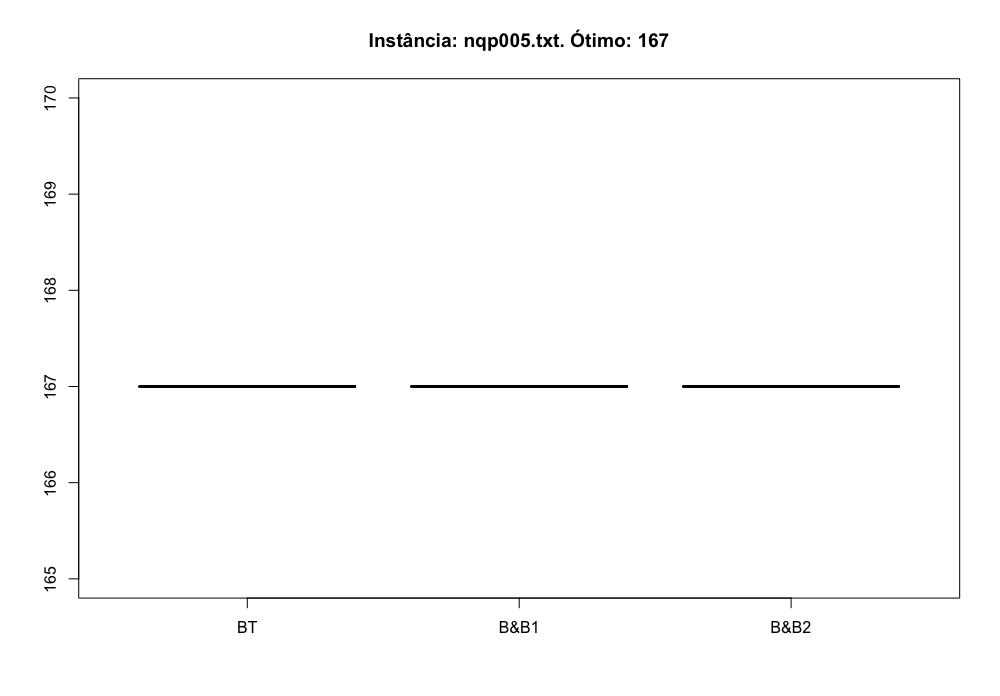
\includegraphics[width=0.9\linewidth]{img/5}
		\caption{BoxPlot da Instância nqp005.txt.}
		\label{fig:5}
	\end{figure}

	A Figura \ref{fig:8} exibe os valores médios obtidos na instância nqp008.txt.

	\begin{figure}[H]
		\centering
		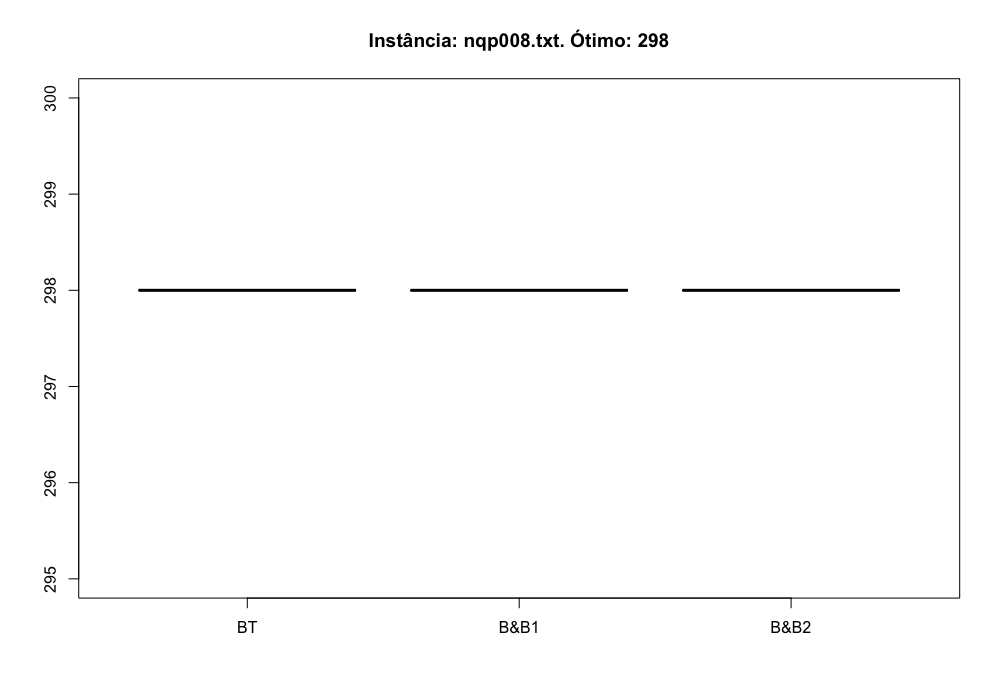
\includegraphics[width=0.9\linewidth]{img/8}
		\caption{BoxPlot da Instância nqp008.txt.}
		\label{fig:8}
	\end{figure}

	A Figura \ref{fig:10} exibe os valores médios obtidos na instância nqp010.txt.

	\begin{figure}[H]
		\centering
		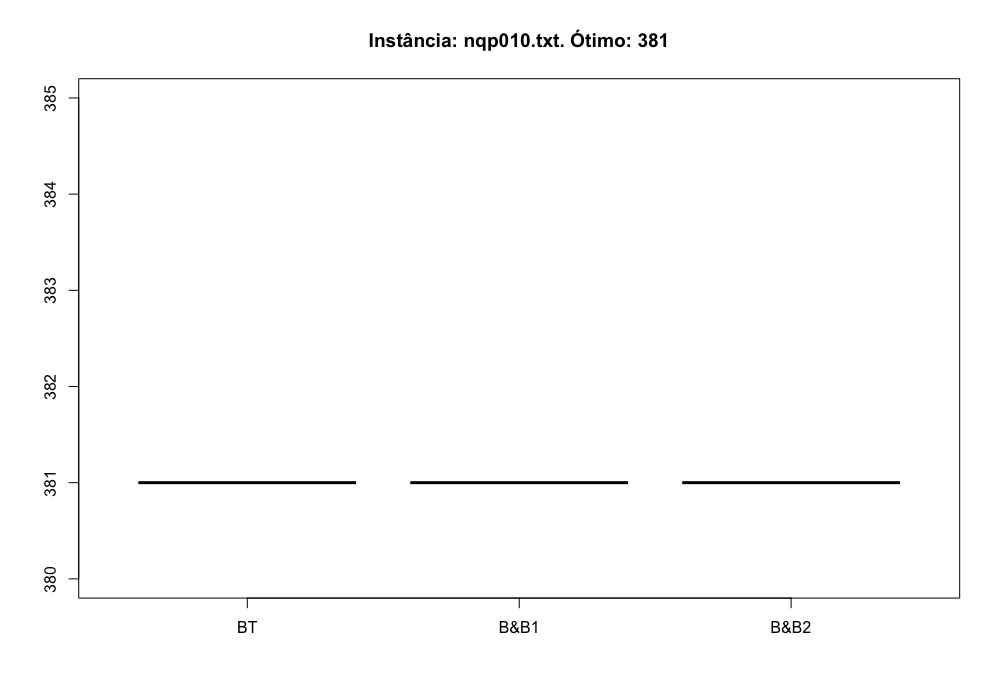
\includegraphics[width=0.9\linewidth]{img/10}
		\caption{BoxPlot da Instância nqp010.txt.}
		\label{fig:10}
	\end{figure}

	A Figura \ref{fig:20} exibe os valores médios obtidos na instância nqp020.txt.

	\begin{figure}[H]
		\centering
		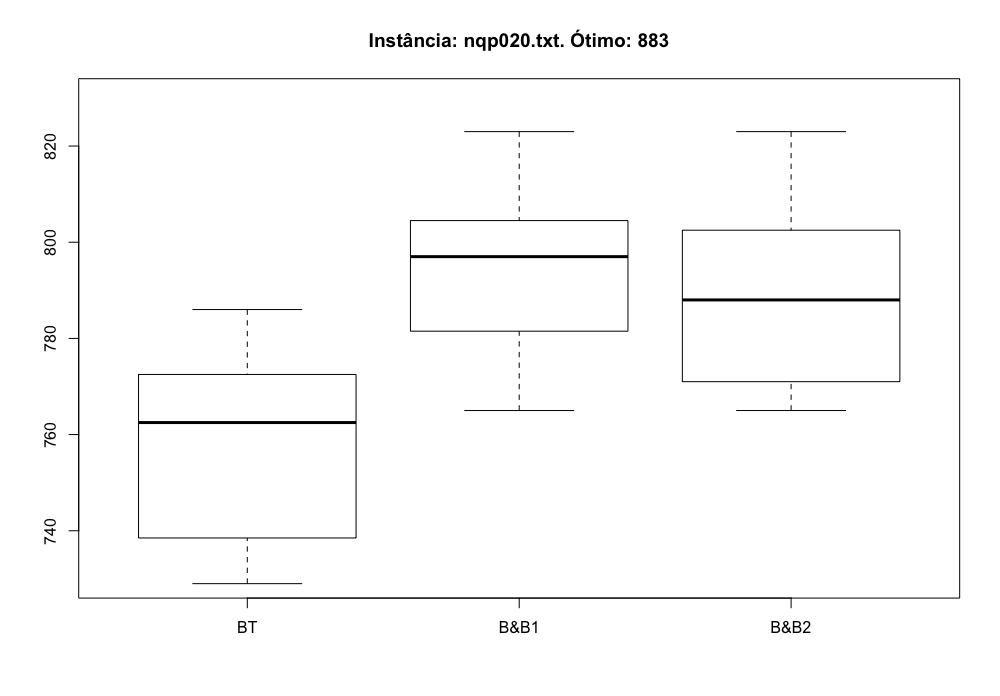
\includegraphics[width=0.9\linewidth]{img/20}
		\caption{BoxPlot da Instância nqp020.txt.}
		\label{fig:20}
	\end{figure}

	A Figura \ref{fig:30} exibe os valores médios obtidos na instância nqp030.txt.

	\begin{figure}[H]
		\centering
		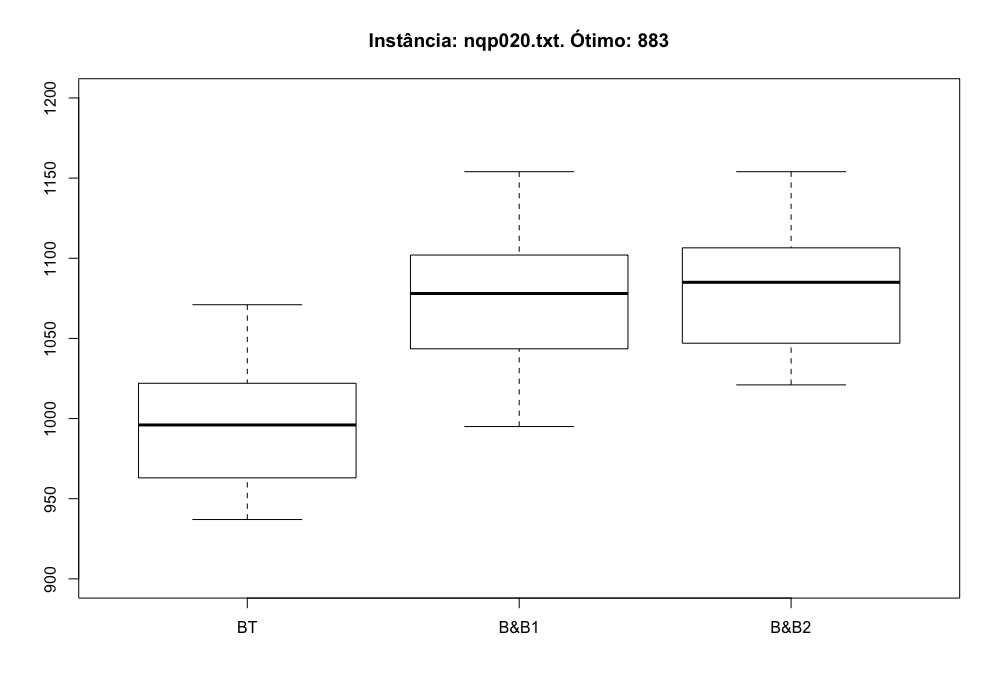
\includegraphics[width=0.9\linewidth]{img/30}
		\caption{BoxPlot da Instância nqp030.txt.}
		\label{fig:30}
	\end{figure}

	A Figura \ref{fig:40} exibe os valores médios obtidos na instância nqp040.txt.

	\begin{figure}[H]
		\centering
		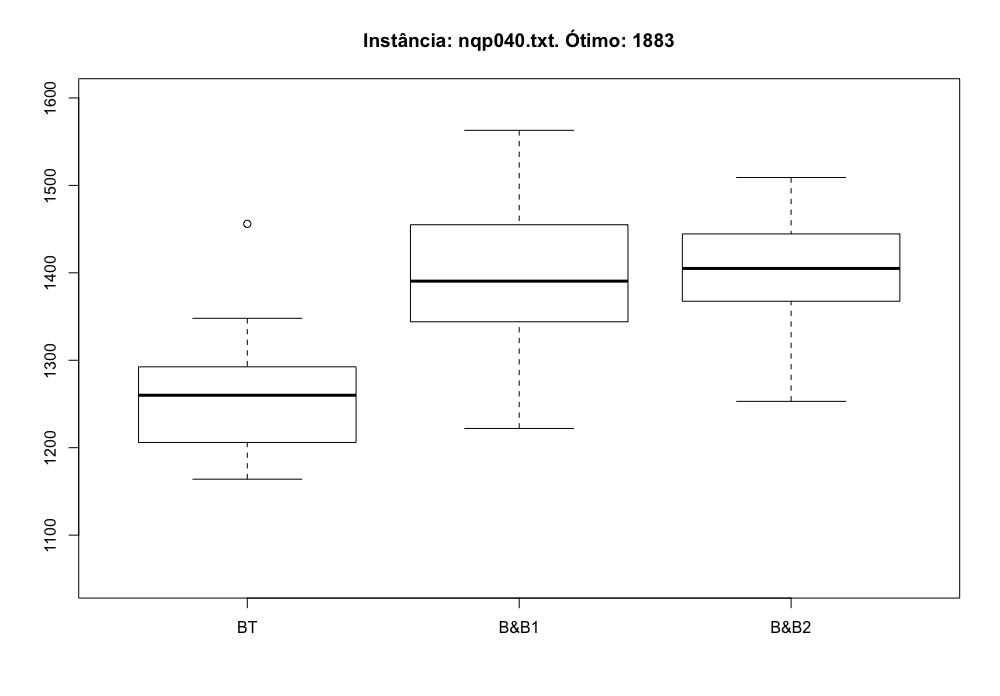
\includegraphics[width=0.9\linewidth]{img/40}
		\caption{BoxPlot da Instância nqp040.txt.}
		\label{fig:40}
	\end{figure}

	A Figura \ref{fig:50} exibe os valores médios obtidos na instância nqp050.txt.

	\begin{figure}[H]
		\centering
		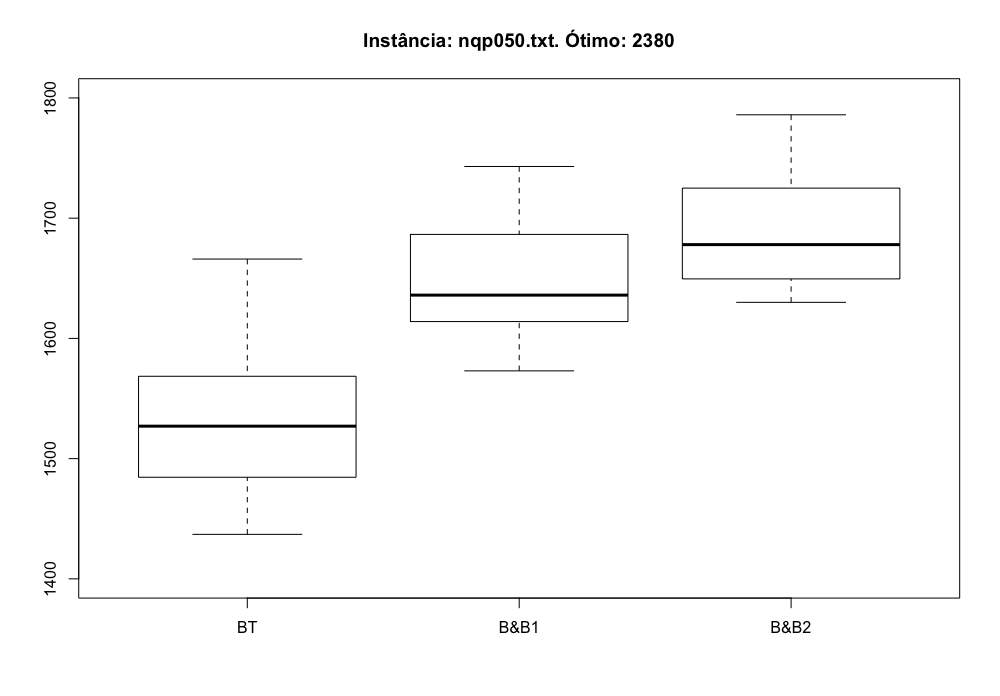
\includegraphics[width=0.9\linewidth]{img/50}
		\caption{BoxPlot da Instância nqp050.txt.}
		\label{fig:50}
	\end{figure}

	A Figura \ref{fig:60} exibe os valores médios obtidos na instância nqp060.txt.

	\begin{figure}[H]
		\centering
		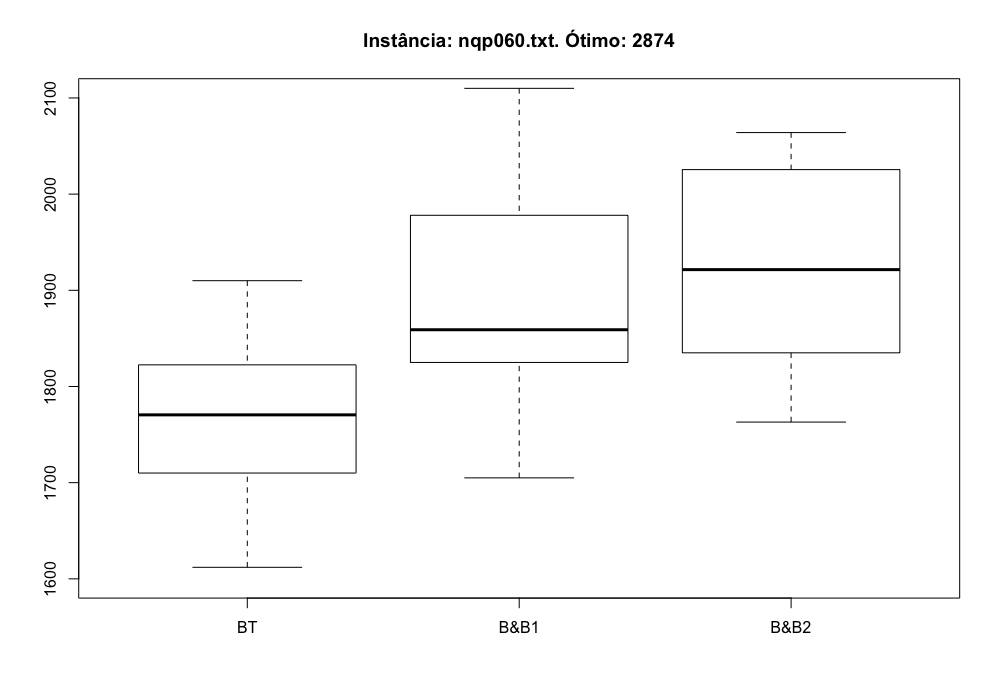
\includegraphics[width=0.9\linewidth]{img/60}
		\caption{BoxPlot da Instância nqp060.txt.}
		\label{fig:60}
	\end{figure}

	A Figura \ref{fig:70} exibe os valores médios obtidos na instância nqp070.txt.

	\begin{figure}[H]
		\centering
		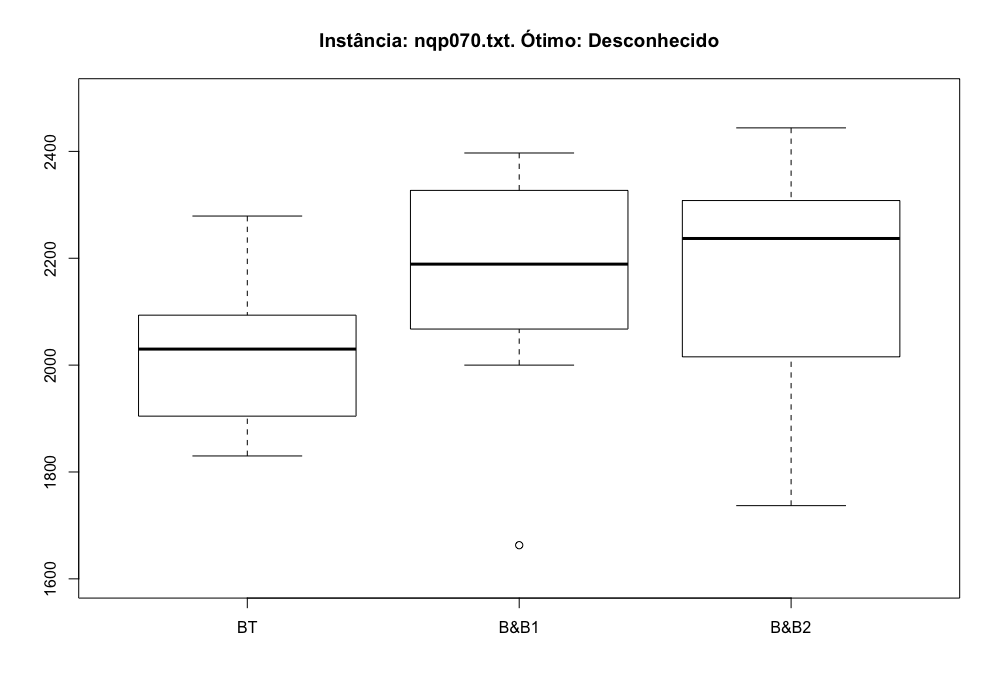
\includegraphics[width=0.9\linewidth]{img/70}
		\caption{BoxPlot da Instância nqp070.txt.}
		\label{fig:70}
	\end{figure}

	A Figura \ref{fig:80} exibe os valores médios obtidos na instância nqp080.txt.

	\begin{figure}[H]
		\centering
		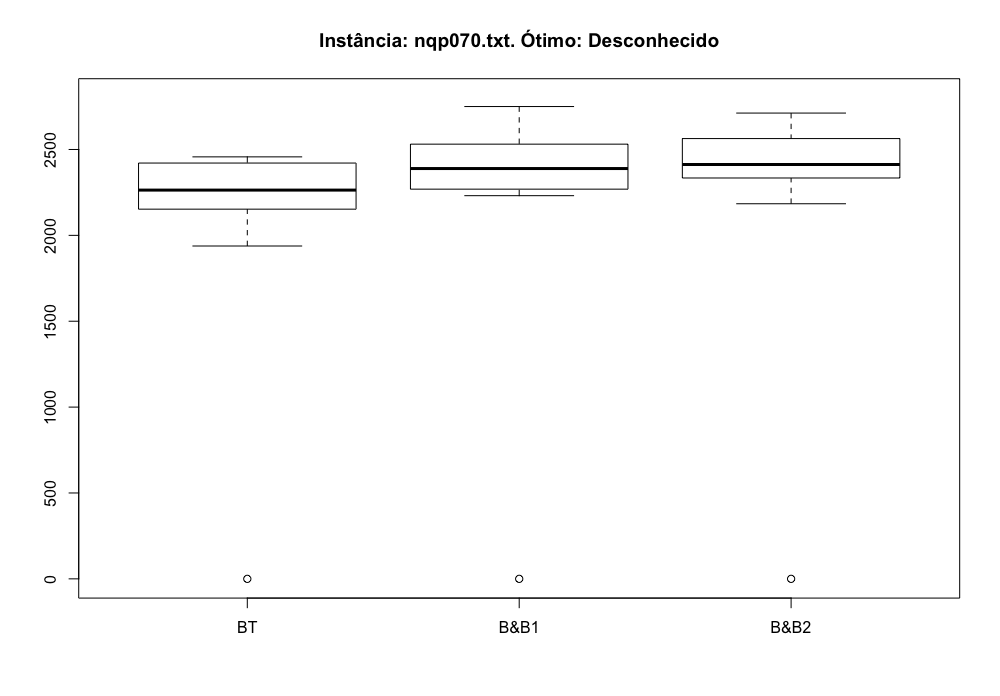
\includegraphics[width=0.9\linewidth]{img/80}
		\caption{BoxPlot da Instância nqp080.txt.}
		\label{fig:80}
	\end{figure}

	A Figura \ref{fig:80-2} exibe somente os maiores valores médios obtidos na instância nqp080.txt, para uma fácil visualização dos melhores valores obtidos.

	\begin{figure}[H]
		\centering
		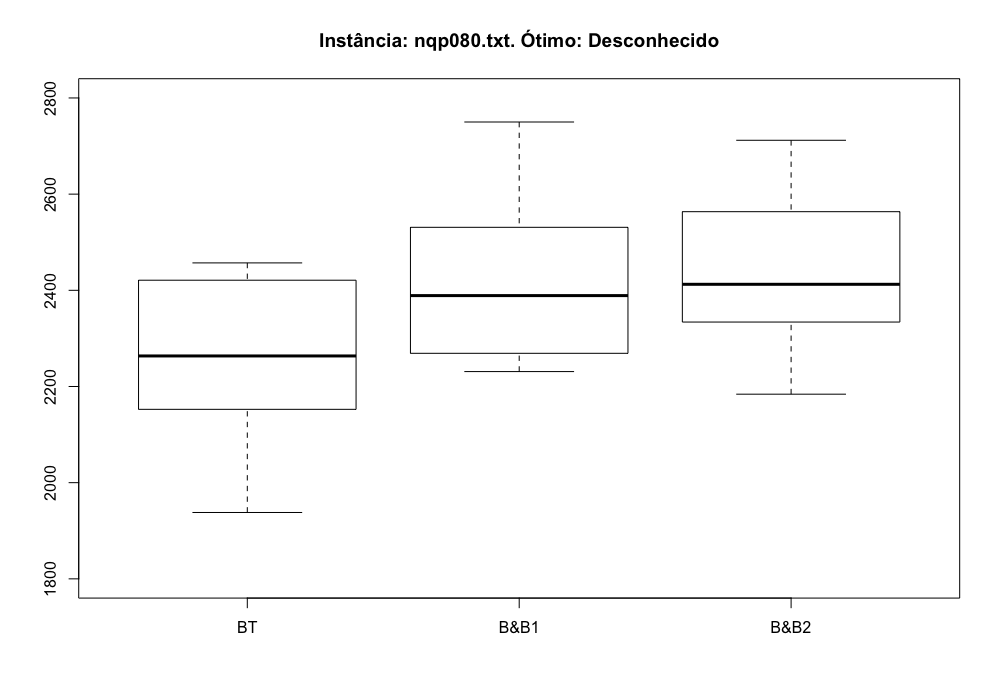
\includegraphics[width=0.9\linewidth]{img/80-2}
		\caption{BoxPlot da Instância nqp080.txt.}
		\label{fig:80-2}
	\end{figure}

	A Figura \ref{fig:90} exibe os valores médios obtidos na instância nqp090.txt.

	\begin{figure}[H]
		\centering
		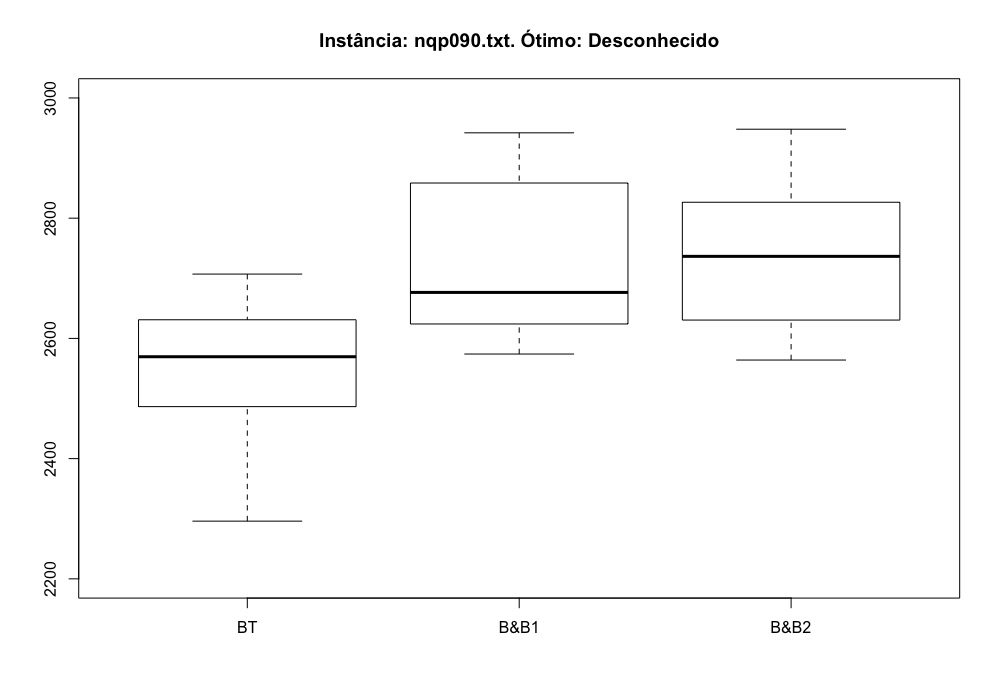
\includegraphics[width=0.9\linewidth]{img/90}
		\caption{BoxPlot da Instância nqp090.txt.}
		\label{fig:90}
	\end{figure}

	A Figura \ref{fig:100} exibe os valores médios obtidos na instância nqp100.txt.

	\begin{figure}[H]
		\centering
		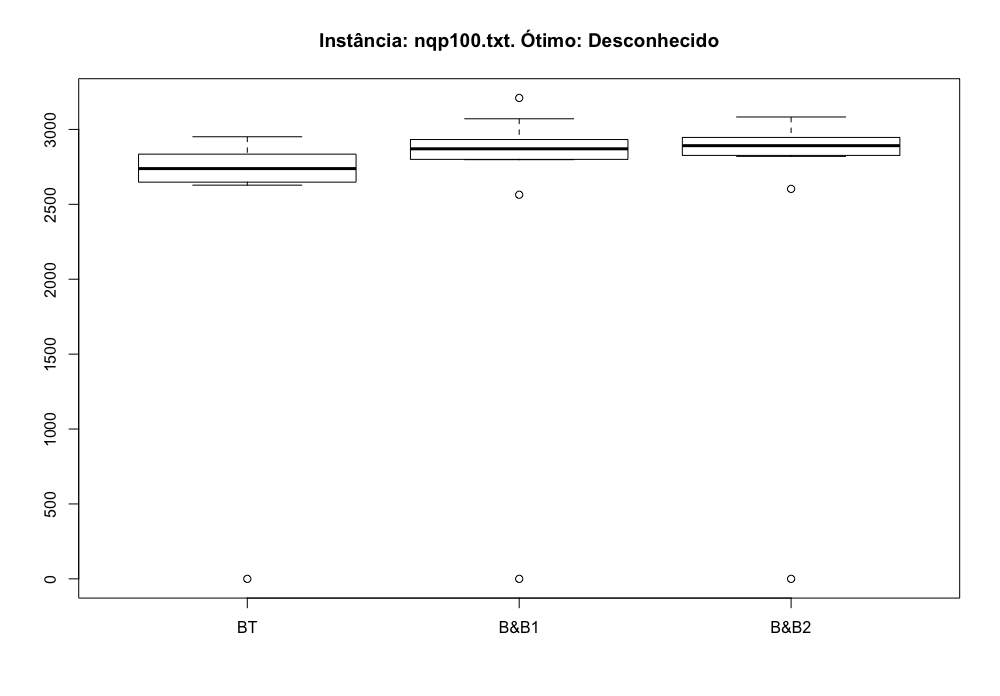
\includegraphics[width=0.9\linewidth]{img/100}
		\caption{BoxPlot da Instância nqp100.txt.}
		\label{fig:100}
	\end{figure}

	A Figura \ref{fig:100-2} exibe somente os maiores valores médios obtidos na instância nqp100.txt, para uma fácil visualização dos melhores valores obtidos.

	\begin{figure}[H]
		\centering
		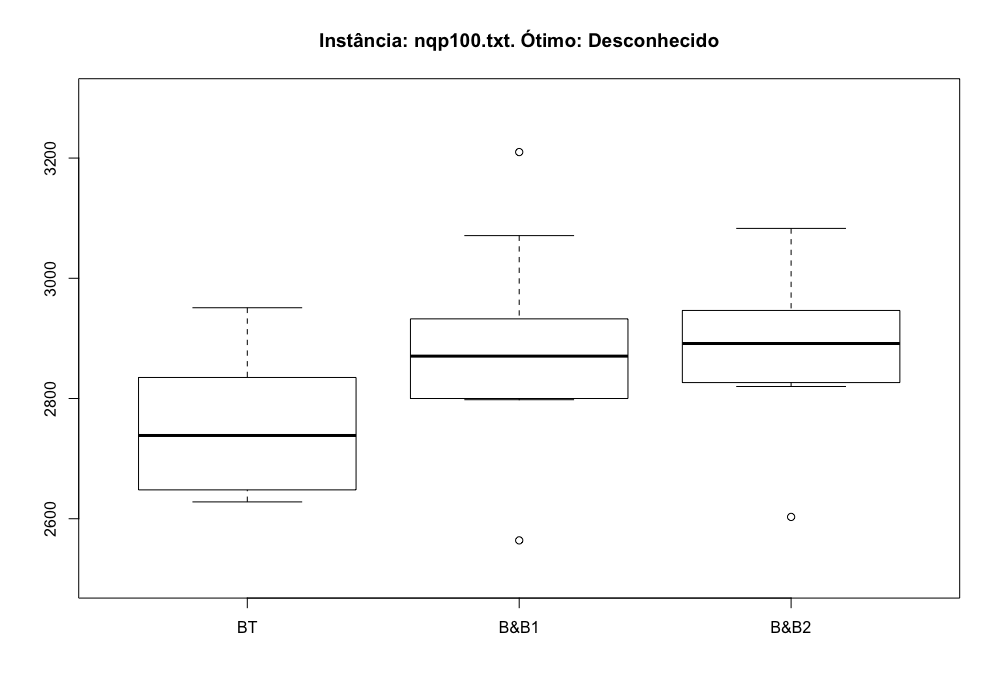
\includegraphics[width=0.9\linewidth]{img/100-2}
		\caption{BoxPlot da Instância nqp100.txt.}
		\label{fig:100-2}
	\end{figure}

	A Figura \ref{fig:200} exibe os valores médios obtidos na instância nqp020.txt.

	\begin{figure}[H]
		\centering
		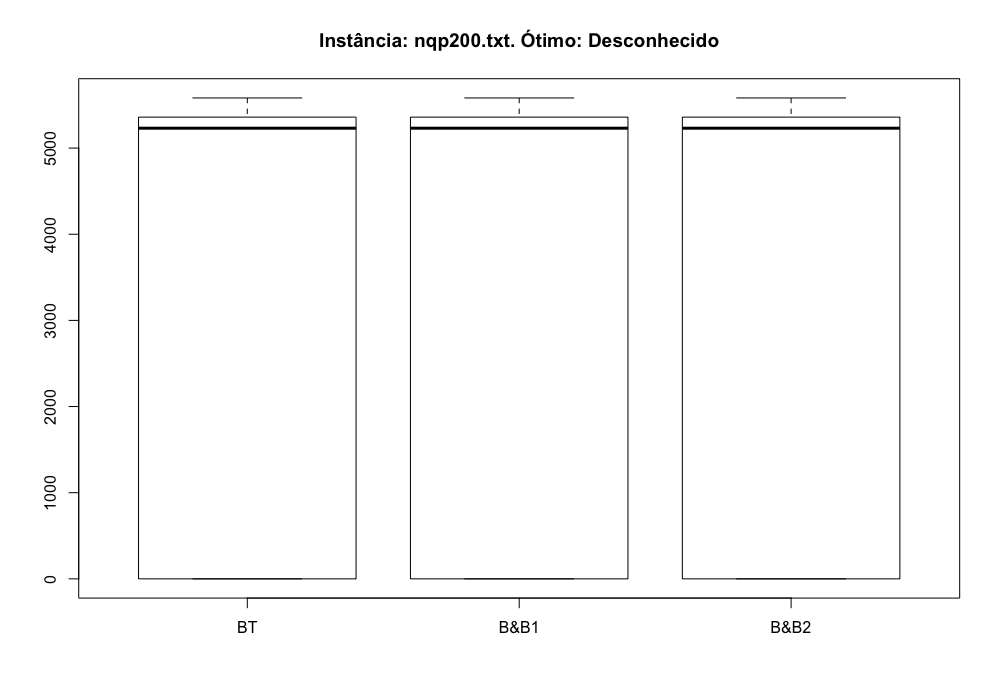
\includegraphics[width=0.9\linewidth]{img/200}
		\caption{BoxPlot da Instância nqp200.txt.}
		\label{fig:200}
	\end{figure}

	A Figura \ref{fig:200-2} exibe somente os maiores valores médios obtidos na instância nqp200.txt, para uma fácil visualização dos melhores valores obtidos.

	\begin{figure}[H]
		\centering
		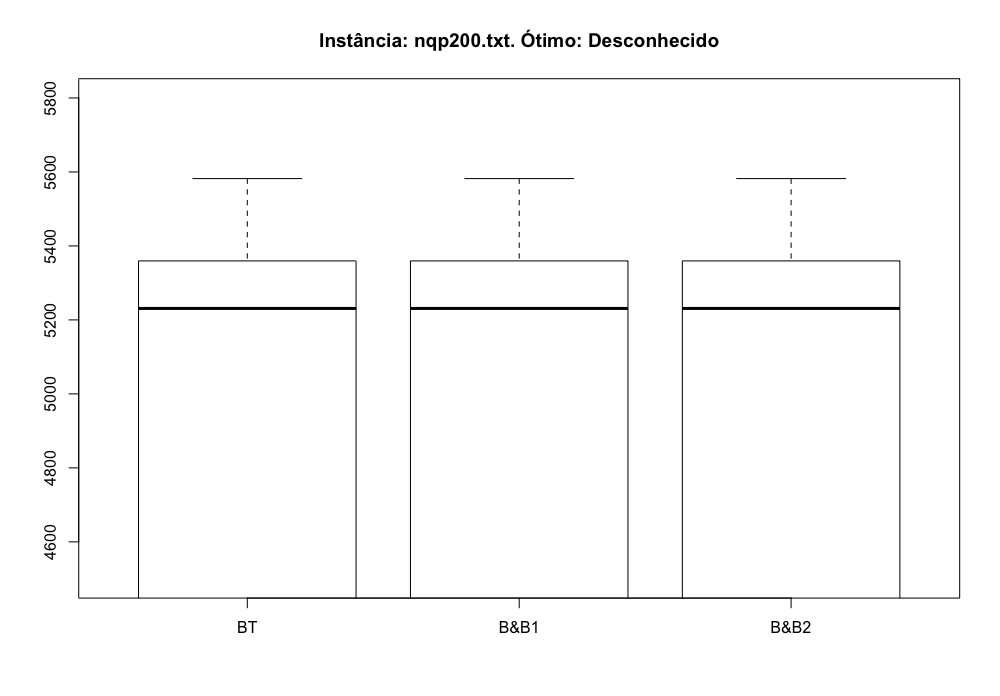
\includegraphics[width=0.9\linewidth]{img/200-2}
		\caption{BoxPlot da Instância nqp200.txt.}
		\label{fig:200-2}
	\end{figure}


\section{Comentários Finais}\label{sec:figs}
	Os algoritmos implementados possuem uma técnica de \textit{análise de soluções parciais} visando a comparação dos \textit{melhores valores} com os \textit{valores atuais} obtidos, cortando ramos que aparentam não ser uma boa estratégia percorrê-los.

	Foram implementados um total de três algoritmos, sendo um com técnica \textit{Backtracking} e outros dois variantes com \textit{Branch and Bound}.

	A primeira implementação utiliza-se de um \textit{Backtracking} simples que verifica todas as soluções possíveis.
	A segunda e terceira é uma variação do primeiro algoritmo adicionando filtros que verificam quão bom é determinado subramo. Foi implementados dois tipos de filtros diferentes e por este motivo, implementou-se dois algoritmos \textit{Branch and Boudn} com o propósito de comparar os resultados dos três algoritmos sobre o mesmo intervalo de tempo.

	É possível ver que o \textit{B\&B 2} obteve melhores resultados na maioria das instâncias, principalmente nas maiores instâncias. Entretanto, não foi um resultado consideravelmente maior já que o algoritmo de \textit{BT} também obteve um resultado tão bom quanto. A análise desses resultados são descritos à seguir.

	Percebeu-se que os algoritmos implementados utilizam de muitas divisões o que torna seu processamento custoso.
	É claro que o compilador realiza otimizações automáticas visando a melhora da execução do código, entretanto, em alto nível, ainda existe forma de aprimorá-lo reduzindo a quantidade de operações repetidas armazenando seu resultado numa variável e utilizá-la quando necessário usando de memória primária para melhorar o tempo de processamento.

	A definição de parâmetros de execução dos filtros também é um item fundamental para uma execução com boas soluções num intervalo de tempo.
	Parâmetros muito restritos podem eliminar soluções que a priori são insuficientes, mas que podem ter bons resultados no decorrer do algoritmo ou até mesmo não encontrando nenhum.
	Já parâmetros com valores relaxados fazem com que o o \textit{Branch and Bound} aproxime-se da técnica \textit{Backtracking} voltando o problema inicial.

	Não somente a variação dos parâmetros, mas também o gerenciamento de novos filtros.
	A adição ou remoção de filtros é uma variação de algoritmo de \textit{Branch and Bound} que também permite filtrar os resultados usando um novo método. Lembrando que qualquer variação realizada, dever-se-á configurar os parâmetros a fim de obter bons resultados em tempo reduzido.

	E possivelmente o fator mais importante a ser trabalhado neste algoritmo seria a execução do algoritmo de força bruta inicial.
	Para casos onde o intervalo de tempo é limitado (tal como este trabalho), o algoritmo de força bruta inicial (\textit{Bactracking}) que é executado em todos os três algoritmos, torna item fundamental para uma boa solução inicial.
	Dependendo do tamanho da instância, seu tempo de execução pode ser ruim o suficiente para utilizar o tempo limite todo para encontrar uma solução inicial válida.
	Observando os resultados da Tabela \ref{tab:resul} e \ref{tab:resulAll} é possível ver que os valores para todos os algoritmos foram exatamente os mesmos na última instância. Pode-se concluir então que no intervalo de tempo de 60 segundos, somente a solução inicial foi executada não permitindo assim a execução do \textit{Branch and Bound}.
	Assim, ter um algoritmo para geração de uma solução inicial rápida, é fundamental para obter um \textit{Branch and Bound} mais eficiente. Com o algoritmo de força bruta inicial mais veloz, é possível que o \textit{Branch and Bound} realize mais podas (mesmo que pequenas) saltando caminhos que possuem soluções ruins e conseguindo resultados melhores ao longo de sua execução.


\section{Código dos Algoritmos}
	Os algoritmos \textit{Shell Script}, \textit{Backtracking}, \textit{Branch and Bound 1} e \textit{Branch and Bound 2} estão distribuídos nas páginas \pageref{cod:shell}, \pageref{cod:bt}, \pageref{cod:bb1} e \pageref{cod:bb1} respectivamente.
	\subsection{\textit{Shell Script}} \label{cod:shell}

\begin{minted}
[
frame=lines,
framesep=2mm,
tabsize=3,
breaklines=true,
baselinestretch=1.2,
linenos,
fontsize=\footnotesize
]{shell}
#!/bin/bash

echo "Quantas iteracoes?"
read quantidade_iteracoes;
echo

eval "rm algori*"
eval "gcc n-Queens-Prize-Backtracking/n-queens-prize-backtracking.c -Ofast -o n-Queens-Prize-Backtracking/n-Queens-Prize-Backtracking"
eval "gcc n-Queens-Prize-BranchAndBound-1/n-queens-prize-branchAndBound-1.c -Ofast -o n-Queens-Prize-BranchAndBound-1/n-Queens-Prize-BranchAndBound-1"
eval "gcc n-Queens-Prize-BranchAndBound-2/n-queens-prize-branchAndBound-2.c -Ofast -o n-Queens-Prize-BranchAndBound-2/n-Queens-Prize-BranchAndBound-2"

instancias=( nqp005.txt nqp008.txt nqp010.txt nqp020.txt nqp030.txt nqp040.txt nqp050.txt nqp060.txt nqp070.txt nqp080.txt nqp090.txt nqp100.txt nqp200.txt )

algoritmos=( n-Queens-Prize-Backtracking n-Queens-Prize-BranchAndBound-1 n-Queens-Prize-BranchAndBound-2 )

for algoritmo in "${algoritmos[@]}"
do
	echo $algoritmo

	for instancia in "${instancias[@]}"
	do
		echo $instancia

		for (( i = 0; i < "$quantidade_iteracoes"; i++ )); do
			echo "$i"

			cmd="./$algoritmo/$algoritmo $instancia $i*1234 60 0"
			date
			echo $cmd
			$cmd
		done
		echo

	done
	echo

done

\end{minted}

	\subsection{\textit{Backtracking}} \label{cod:bt}



\begin{minted}
[
frame=lines,
framesep=2mm,
tabsize=3,
breaklines=true,
baselinestretch=1.2,
linenos,
fontsize=\footnotesize
]{c}
#include <stdio.h>
#include <stdlib.h>
#include <time.h>

// variável global sobre a quantidade de colunas/linhas da matriz
int global_tamanho_matriz = -1;
// variável que ativa impressoes na tela
char global_imprime_tela_ativado = 0;

// Variáveis de tempo para cálculo do intervalo de tempo de execução
time_t endwait, start;


/*
 * Estrutura que representa um tabuleiro.
 *
 * Um ponteiro para um vetor de onde representa cada posicao da rainha na coluna
 * O valor de prêmrio do tabuleiro no estado atual
 */
typedef struct Struct_Tabuleiro {
	int * colunas;
	int   premio;
} Tabuleiro;


/*
 * Estrutura de representação de Fila
 *
 * Esta fila é utilizada para organizar a ordem de seleção das rainhas
 */
typedef struct Struct_Fila {
	int           lugar; // Posição da rainha
	struct Struct_Fila * proximo;
} Fila;



/*
 * Procedimento que verifica se a fila passada por parâmetro está vazia.
 *
 * Retorna valores boleanos
 */
char Fila_Esta_Vazia(Fila * f) {
	if (f == NULL) {
		return 1;
	} else
		return 0;
}



/*
 * Procedimento que adiciona um novo valor à fila
 */
void Enfilera(Fila ** f, int l) {
	Fila * atual = 0, * novo = 0;

	// Cria um novo nó e adiciona informações
	novo = calloc(1, sizeof(Fila));
	novo->lugar = l;
	novo->proximo = NULL;


	// Se a fila estiver vazia, coloca na cabeça
	if (Fila_Esta_Vazia(*f)) {

		* f = novo;

	} else {
		// Caso contrário, coloca na calda

		atual = * f;

		while(atual->proximo != NULL) {
			atual = atual->proximo;
		}

		atual->proximo = novo;
	}
}



/*
 * Procedimento que realiza a retirada de um elemento da fila seguindo sua natureza
 */
int Desenfilera(Fila ** f) {
	Fila * retirar = 0, * fila = * f;
	int posicao = 0;

	// Se a fila estiver vazia, informa erro e termina o programa
	if (Fila_Esta_Vazia(*f)) {
		printf("\n\n[ERRO] Impossível retirar de uma fila vazia. \tFinalizando o programa.");
		return -1;
	} else {
		// caso contrário, retira o primeiro elemento.
		posicao = fila->lugar;
		retirar = fila;

		fila = fila->proximo;

		free(retirar);

		*f = fila;

		return posicao;
	}
}



/*
 * Procedimento que realiza o processo de retirar todos os elementos da fila
 */
void Desaloca_Fila(Fila ** f) {
	Fila * retirar = 0;

	// Retira todos os elementos da fila
	while (*f != NULL) {
		retirar = *f;

		*f = (*f)->proximo;

		free (retirar);
	}

}



/*
 * Procedimento para impressão da Fila na tela
 */
void Imprime_Fila(Fila * f) {
	Fila * atual = f;

	if (global_imprime_tela_ativado) {

		printf("\n\n\t\t");
		while (atual != NULL) {
			printf("%d -> ", atual->lugar);
			atual = atual->proximo;
		}
		printf("NULL");

		fflush(stdout);
	}
}



/*
 * Procedimento responsável por gerar uma fila de posições de rainhas em ordem aleatória.
 *
 * Primeiro cria-se um vetor com os valores de 1..n ordenado simbolizando a ordem das rainhas.
 * Em seguida, é gerado dois valores inteiros posicao1 e posicao2 de forma aleatória e estes
 *		são utilizados para a comutação dos valores situados em vetor[posicao1] e vetor[posicao2]
 * No final de algumas iterações, estes respectivos valores já desordenados são copiados para
 *		a fila para que o algoritmo use.
 */
Fila * Cria_Fila_Aleatoria() {
	Fila * f = 0, * cabeca = 0;

	int vetor_valores_fila [global_tamanho_matriz],
			i = 0,
			permutacoes = global_tamanho_matriz * 10,
			posicao1 = 0, posicao2 = 0, temp = 0;

	// Cria-se um vetor com valores ordenados de 1..n_rainhas
	for (i = 0; i < global_tamanho_matriz; i++) {
		vetor_valores_fila[i] = i;
	}

	// Realiza várias permutações dos valores deste vetor de acordo com os dois índices gerados
		// Realiza-se global_tamanho_matriz * 10 permutações
	i = 0;
	while (i < permutacoes) {
		// Gera primeiro índice
		posicao1 = rand() % global_tamanho_matriz;

		// Gera segundo índice
		posicao2 = rand() % global_tamanho_matriz;

		// Realiza a comutação dos valores dos respectivos índices
		temp = vetor_valores_fila[posicao1];
		vetor_valores_fila[posicao1] = vetor_valores_fila[posicao2];
		vetor_valores_fila[posicao2] = temp;

		i++;
	}

	// Aloca a fila e adiciona os valores após realizar a desordem
	cabeca = calloc(1, sizeof(Fila));

	f = cabeca;

	// Copia os valores do vetor para a fila
	i = 0;
	while (i < global_tamanho_matriz - 1) {

		f->lugar = vetor_valores_fila[i];

		f->proximo = calloc(1, sizeof(Fila));

		f = f->proximo;

		i++;
	}

	f->lugar = vetor_valores_fila[i];

	f->proximo = NULL;

	// Retorna a fila desordenada
	return cabeca;
}



/*
 * Procedimento para retorndo do de prêmio específico de uma célula
 */
int Retorna_Premio(int * premios, int linha, int coluna) {

	// Acessa o vetor como se fosse uma matriz comum nxn.
	return premios[linha * global_tamanho_matriz + coluna];
}



/*
 * Procedimento para realizar a leitura dos arquivo prêmio
 *
 * Este também armazena o maior premio lido e o retorna.
 */
void Le_Premios(char * diretorio, int ** premios){
	FILE * file = 0;
	int i = 0;
	int premio_lido = 0;
	int quantidade_celulas = 0;

	// Abre o arquivo de prêmios em forma de leitura
	file = fopen(diretorio, "r");

	// Verifica se a abertura foi feita com sucesso
	if (file != NULL) {

		//lê a primeira informação (quantas linhas existem)
		fscanf(file, "%d", &global_tamanho_matriz);
		if (global_imprime_tela_ativado)
			printf("\n[INFO] Quantidade de colunas do tabuleiro = %d.\n", global_tamanho_matriz);

		// Se o valor de tamanho da matriz for um valor válido
		if (global_tamanho_matriz > 0) {

			quantidade_celulas = global_tamanho_matriz * global_tamanho_matriz;

			// Aloca a matriz de prêmios
			* premios = calloc(quantidade_celulas, sizeof(int));

			// Começa a coleta dos prêmios
			fscanf(file, "%d", &premio_lido);

			// Salvas os prêmios e coleta o próximo
			while(i < quantidade_celulas) {

				if (global_imprime_tela_ativado) {
					// Imprime na tela o prêmio lido
					printf("\n[INFO] Lendo premio [%d,%d] = %d.", i / global_tamanho_matriz + 1, i % global_tamanho_matriz + 1, premio_lido);
					fflush(stdout);
				}

				// Salva no vetor
				(*premios)[i++] = premio_lido;

				// Lê o próximo prêmio
				fscanf(file, "%d", &premio_lido);
			}
		} else {
			// Informa Erro
			printf("\n[ERRO] Quantidade de rainhas insuficiente!\n\n");
			exit(-1);
		}

		// Fecho o arquivo
		fclose(file);
	}
	else {
		// Informa Erro
		printf("\n[ERRO] Falha na leitura do arquivo de configuração!\n\n");
		exit(-1);
	}
}



/*
 * Como utiliza-se uma estrutura fila com todas as opções e sem repetição, não
 *		existe a possibilidade de duas rainhas ficarem numa mesma linha
 *		vertical, horizontal (isso pois os valores não se repetem).
 *
 * Com isso, basta verificar se as diagonais estão conflitando.
 */
char Posicao_Eh_Valida(Tabuleiro t, int col, int pos) {
	int i = 0;
	char esquerda_diagonal = 0, direita_diagonal = 0;

	// Inicializa dizendo que as diagonais não estão ocupadas
	esquerda_diagonal = direita_diagonal = 1;

	// Da posição da rainha até a coluna 0, faça:
	i = col;
	while (i > 0) {

		// Verifica:
		//		Diagonal esquerda-direita
		if (t.colunas[col - i]  == pos + i) {
			esquerda_diagonal = 0;

		// Verifica:
		//		Diagonal direita-esquerda
		} else
			if (t.colunas[col - i] == pos - i) {
			direita_diagonal = 0;
		}

		// Verifica validade
		// Caso alguma diagonal já esteja ocupada, aborta o procedimento
			// informando que esta posição é inválida
		if (esquerda_diagonal == 0 || direita_diagonal == 0) {
			return 0;
		}

		i--;
	}

	// Verifica validade das diagonais
	if (esquerda_diagonal == 1 && direita_diagonal == 1)
		return 1;
	else
		return 0;
}



/*
 * Procedimento que copia os dados de um tabuleiro para outro.
 *
 * Este procedimento é utilizando quando encontra-se um novo valor de prêmio maior
 *		que o atual e assim, realiza-se a substituição do tabuleiro antigo pelo novo
 *		encontrado.
 */
void Copia_Novo_Tabuleiro(Tabuleiro tabuleiro_atual, Tabuleiro * tabuleiro_maior) {
	int i = 0;

	tabuleiro_maior->premio           = tabuleiro_atual.premio;

	for (i = 0; i < global_tamanho_matriz; i++) {
		tabuleiro_maior->colunas[i]   = tabuleiro_atual.colunas[i];
	}
}



/*
 * Procedimento que adiciona uma nova rainha no tabuleiro já calculando o prêmio desta.
 *
 * Este procedimento não precisa verificar a validade da posição já que este já foi calculado
 *		quando a rainha foi selecionada.
 */
void Adiciona_Rainha_Tabuleiro_Calculando_Premio(Tabuleiro * t, int posicao,  int r, int * premios) {

	t->premio += Retorna_Premio(premios, r, posicao);
	t->colunas[posicao] = r;
}



/*
 * Procedimento que retira a rainha do tabuleiro calculando o novo prêmio
 */
void Retira_Rainha_Tabuleiro_Calculando_Premio(Tabuleiro * t, int posicao, int r, int * premios) {
	t->premio -= Retorna_Premio(premios, r, posicao);
	t->colunas[posicao] = -1;
}



/*
 * Procedimento que inicializa um novo tabuleiro
 */
Tabuleiro * Cria_Tabuleiro(){
	int i = 0;
	Tabuleiro * t = 0;

	t = calloc(1, sizeof(Tabuleiro));
	t->colunas = calloc(global_tamanho_matriz, sizeof(int));

	for (i = 0; i < global_tamanho_matriz; i++)
		t->colunas[i] = -1;

	return t;
}



/*
 * Procedimento que imprime o tabuleiro junto com os prêmios
 */
void Imprime_Tabuleiro (Tabuleiro t, Tabuleiro maior, int * premios) {
	int i = 0, j = 0;

	if (global_imprime_tela_ativado) {

		printf("\n");

		for (i = 0; i < global_tamanho_matriz; i++) {
				printf("\n\t");
			for (j = 0; j < global_tamanho_matriz * 2; j++) {
				if ( j < global_tamanho_matriz) {
					if (i == t.colunas[j])
						printf("%3d ", i);
					else
						printf(" -1 ");
				}
				else {
					if (j == global_tamanho_matriz)
						printf("\t\t");
					printf("%3d ", premios[i * global_tamanho_matriz + j - global_tamanho_matriz]);
				}

			}

			fflush(stdout);
		}

		printf("\tPremio_Atual: %d;\tMaior_Premio: %d.", t.premio, maior.premio);

		fflush(stdout);
	}
}


/*
 * Procedimento que imprime o tabuleiro, junto com os prêmios informando fim da execução
 */
void Imprime_Tabuleiro_Final (Tabuleiro maior, int * premios) {
	int i = 0, j = 0;
	FILE * saida = 0;

	if (global_imprime_tela_ativado) {

		printf("\n\n[INFO] Resultado Final do Processamento:");

		for (i = 0; i < global_tamanho_matriz; i++) {
				printf("\n\t");
			for (j = 0; j < global_tamanho_matriz * 2; j++) {
				if ( j < global_tamanho_matriz) {
					if (i == maior.colunas[j])
						printf("%3d ", i);
					else
						printf(" -1 ");
				}
				else {
					if (j == global_tamanho_matriz)
						printf("\t\t");
					printf("%3d ", premios[i * global_tamanho_matriz + j - global_tamanho_matriz]);
				}
			}

			fflush(stdout);
		}

		printf("\tPremio: %d.",maior.premio);
		printf("\n[INFO] Resultado Final do Processamento.\n");
	} else {
		saida = fopen("algoritmo0.txt", "a");

		if (saida) {
			fprintf(saida, "%d\n", maior.premio);
		}

		fclose(saida);
	}

	fflush(stdout);
}



/*
 * Procedimento que libera memória
 */
 void Desaloca_Tabuleiro (Tabuleiro ** f) {
	if (*f != 0) {
		free((*f)->colunas);
		free(*f);
	}
 }



/*
 * Procedimento que libera memória
 */
void Desaloca_Premios (int ** premios) {
	if (*premios != 0)
		free(*premios);
}



/*
 * Método de branch and bound desenvolvido
 */
void n_Rainhas_Prize(int coluna_atual, Tabuleiro * tabuleiro_atual, Tabuleiro * tabuleiro_maior, Fila ** posicoes_restantes, int * premios) {
	int iteracoes = 0, linha_atual_temp = 0;

	// Recebe o tempo atual.
	start = time(NULL);

	// Verifica se o tempo excedeu o liminte estabelecido.
	if (start > endwait) {
		// Se sim, cancela totalmente a continuação da recursão
		return ;
	}


	// Varre a fila com os valores que sobraram
		// A cada recursão, um item é retirado

	// Caso tenha percorrido todas as rainhas deste contexto de recursão,
		// o while será impedido de ser executando forçando a realizar o
		// retorno à um nível acima de recursao
	while (iteracoes < global_tamanho_matriz - coluna_atual) {

		Imprime_Fila(* posicoes_restantes);
		Imprime_Tabuleiro(*tabuleiro_atual, *tabuleiro_maior, premios);

		// Retira um item da fila e salva numa variável local
		linha_atual_temp = Desenfilera( posicoes_restantes );

			printf("\nALERTA%d\n", linha_atual_temp);
		if (linha_atual_temp == -1) {
			Desaloca_Premios(&premios);

			Desaloca_Tabuleiro(&tabuleiro_maior);
			Desaloca_Tabuleiro(&tabuleiro_atual);
			exit(-1);
		}

		Imprime_Fila(* posicoes_restantes);
		if (global_imprime_tela_ativado) {
			printf("\t\tBuffer_Atual: %d", linha_atual_temp);
			fflush(stdout);
		}


		// Testa a validade da rainha retirada no momento
			// Se for posição válida realizará o processamento desta
			// Caso contrário, ela será posta no final da fila=
		if(Posicao_Eh_Valida(*tabuleiro_atual, coluna_atual, linha_atual_temp)) {

			// Adiciona a rainha no tabuleiro calculando o prêmio com sua inclusão
			Adiciona_Rainha_Tabuleiro_Calculando_Premio(tabuleiro_atual, coluna_atual, linha_atual_temp, premios);

			Imprime_Tabuleiro(*tabuleiro_atual, *tabuleiro_maior, premios);


			// Se a fila estiver vazia, significa que acabou de ser gerado uma solução
				// válida.
			// Assim, será verificado se o prêmio é melhor que o atual.
			if (Fila_Esta_Vazia(* posicoes_restantes)) {

				if (tabuleiro_atual->premio > tabuleiro_maior->premio) {

					if (global_imprime_tela_ativado)
						printf("\n\n[INFO] Novo Recorde Encontrado!");
					Copia_Novo_Tabuleiro(*tabuleiro_atual, tabuleiro_maior);

					Imprime_Tabuleiro(*tabuleiro_atual, *tabuleiro_maior, premios);
				}


				Imprime_Fila(*posicoes_restantes);

				// Após chegar na folha, a recursão é revertida até que encontre
					// uma próxima solução pra explorar.
				Enfilera(posicoes_restantes, linha_atual_temp);

				Imprime_Fila(*posicoes_restantes);

				// Como mencionado, a raínha é posta novamente na fila para a procura
					// de novas soluções
				Retira_Rainha_Tabuleiro_Calculando_Premio(tabuleiro_atual, coluna_atual, linha_atual_temp, premios);


				return ;


			// Se não for a última rainha, então realiza as análises de bound
			} else {

				n_Rainhas_Prize(coluna_atual + 1, tabuleiro_atual, tabuleiro_maior, posicoes_restantes, premios);


				Enfilera(posicoes_restantes, linha_atual_temp);

				Retira_Rainha_Tabuleiro_Calculando_Premio(tabuleiro_atual, coluna_atual, linha_atual_temp, premios);

				Imprime_Fila(*posicoes_restantes);

				iteracoes++;
			} // if


		// Se a posição escolhida não for válida
		} else {

			if(global_imprime_tela_ativado) {
				printf("\n[INFO] Posição Inválida. Retornando o valor %d à fila", linha_atual_temp);
				fflush(stdout);
			}

			// Readiciona-la no final da fila
			Enfilera(posicoes_restantes, linha_atual_temp);

			Imprime_Fila(*posicoes_restantes);

			// Passa pra próxima rainha
			iteracoes++;

		} // if

	} // While


	// Após ter percorrido todos as soluções deste nível e seus subníveis
		// é retornado um nível para continuar a busca.

	if(global_imprime_tela_ativado)
		printf("\n[INFO] Saindo do nível %d", coluna_atual);

	return ;

}


int main(int argc, char** argv) {
	int * premios = 0;
	char * diretorio = 0;
	Tabuleiro * tabuleiro_atual = 0, * tabuleiro_maximo_encontrado = 0;
	Fila * fila_rainhas = 0;
	time_t seconds = 0;

	if (argc != 4) {
		diretorio = argv[1];
		srand(atoi(argv[2]));
		seconds = atoi(argv[3]);
		global_imprime_tela_ativado = atoi(argv[4]);

	} else {
		exit(-1);
	}

	Le_Premios(diretorio, &premios);

	tabuleiro_atual = Cria_Tabuleiro();
	tabuleiro_maximo_encontrado = Cria_Tabuleiro();

	fila_rainhas = Cria_Fila_Aleatoria();

	start = time(NULL);

	endwait = start + seconds;


	n_Rainhas_Prize(0, tabuleiro_atual, tabuleiro_maximo_encontrado, &fila_rainhas, premios);


	Imprime_Tabuleiro_Final(*tabuleiro_maximo_encontrado, premios);

	Desaloca_Fila(&fila_rainhas);
	Desaloca_Premios(&premios);
	Desaloca_Tabuleiro(&tabuleiro_maximo_encontrado);
	Desaloca_Tabuleiro(&tabuleiro_atual);

	return (EXIT_SUCCESS);
}

\end{minted}

	\subsection{\textit{Branch and Bound} 1} \label{cod:bb1}

\begin{minted}
[
frame=lines,
framesep=2mm,
tabsize=3,
breaklines=true,
baselinestretch=1.2,
linenos,
fontsize=\footnotesize
]{c}
#include <stdio.h>
#include <stdlib.h>
#include <time.h>

// variável global sobre a quantidade de colunas/linhas da matriz
int global_tamanho_matriz = -1;
// variável que ativa impressoes na tela
char global_imprime_tela_ativado = 0;

// Variáveis de tempo para cálculo do intervalo de tempo de execução
time_t endwait, start;


/*
 * Estrutura que representa um tabuleiro.
 *
 * Um ponteiro para um vetor de onde representa cada posicao da rainha na coluna
 * O valor de prêmrio do tabuleiro no estado atual
 */
typedef struct Struct_Tabuleiro {
	int * colunas;
	int   premio;
} Tabuleiro;


/*
 * Estrutura de representação de Fila
 *
 * Esta fila é utilizada para organizar a ordem de seleção das rainhas
 */
typedef struct Struct_Fila {
	int           lugar; // Posição da rainha
	struct Struct_Fila * proximo;
} Fila;



/*
 * Procedimento que verifica se a fila passada por parâmetro está vazia.
 *
 * Retorna valores boleanos
 */
char Fila_Esta_Vazia(Fila * f) {
	if (f == NULL) {
		return 1;
	} else
		return 0;
}



/*
 * Procedimento que adiciona um novo valor à fila
 */
void Enfilera(Fila ** f, int l) {
	Fila * atual = 0, * novo = 0;

	// Cria um novo nó e adiciona informações
	novo = calloc(1, sizeof(Fila));
	novo->lugar = l;
	novo->proximo = NULL;


	// Se a fila estiver vazia, coloca na cabeça
	if (Fila_Esta_Vazia(*f)) {

		* f = novo;

	} else {
		// Caso contrário, coloca na calda

		atual = * f;

		while(atual->proximo != NULL) {
			atual = atual->proximo;
		}

		atual->proximo = novo;
	}
}



/*
 * Procedimento que realiza a retirada de um elemento da fila seguindo sua natureza
 */
int Desenfilera(Fila ** f) {
	Fila * retirar = 0, * fila = * f;
	int posicao = 0;

	// Se a fila estiver vazia, informa erro e termina o programa
	if (Fila_Esta_Vazia(*f)) {
		printf("\n\n[ERRO] Impossível retirar de uma fila vazia.");
		return -1;

	} else {
		// caso contrário, retira o primeiro elemento.
		posicao = fila->lugar;
		retirar = fila;

		fila = fila->proximo;

		free(retirar);

		*f = fila;

		return posicao;
	}
}



/*
 * Procedimento que realiza o processo de retirar todos os elementos da fila
 */
void Desaloca_Fila(Fila * f) {
	Fila * retirar = 0;

	// Retira todos os elementos da fila
	while (f != NULL) {
		retirar = f;

		f = f->proximo;

		free (retirar);
	}

}



/*
 * Procedimento para impressão da Fila na tela
 */
void Imprime_Fila(Fila * f) {
	Fila * atual = f;

	if (global_imprime_tela_ativado) {

		printf("\n\n\t\t");
		while (atual != NULL) {
			printf("%d -> ", atual->lugar);
			atual = atual->proximo;
		}
		printf("NULL");

		fflush(stdout);
	}
}



/*
 * Procedimento responsável por gerar uma fila de posições de rainhas em ordem aleatória.
 *
 * Primeiro cria-se um vetor com os valores de 1..n ordenado simbolizando a ordem das rainhas.
 * Em seguida, é gerado dois valores inteiros posicao1 e posicao2 de forma aleatória e estes
 *		são utilizados para a comutação dos valores situados em vetor[posicao1] e vetor[posicao2]
 * No final de algumas iterações, estes respectivos valores já desordenados são copiados para
 *		a fila para que o algoritmo use.
 */
Fila * Cria_Fila_Aleatoria() {
	Fila * f = 0, * cabeca = 0;

	int vetor_valores_fila [global_tamanho_matriz],
			i = 0,
			permutacoes = global_tamanho_matriz * 10,
			posicao1 = 0, posicao2 = 0, temp = 0;

	// Cria-se um vetor com valores ordenados de 1..n_rainhas
	for (i = 0; i < global_tamanho_matriz; i++) {
		vetor_valores_fila[i] = i;
	}

	// Realiza várias permutações dos valores deste vetor de acordo com os dois índices gerados
		// Realiza-se global_tamanho_matriz * 10 permutações
	i = 0;
	while (i < permutacoes) {
		// Gera primeiro índice
		posicao1 = rand() % global_tamanho_matriz;

		// Gera segundo índice
		posicao2 = rand() % global_tamanho_matriz;

		// Realiza a comutação dos valores dos respectivos índices
		temp = vetor_valores_fila[posicao1];
		vetor_valores_fila[posicao1] = vetor_valores_fila[posicao2];
		vetor_valores_fila[posicao2] = temp;

		i++;
	}

	// Aloca a fila e adiciona os valores após realizar a desordem
	cabeca = calloc(1, sizeof(Fila));

	f = cabeca;

	// Copia os valores do vetor para a fila
	i = 0;
	while (i < global_tamanho_matriz - 1) {

		f->lugar = vetor_valores_fila[i];

		f->proximo = calloc(1, sizeof(Fila));

		f = f->proximo;

		i++;
	}

	f->lugar = vetor_valores_fila[i];

	f->proximo = NULL;

	// Retorna a fila desordenada
	return cabeca;
}



/*
 * Procedimento para retorndo do de prêmio específico de uma célula
 */
int Retorna_Premio(int * premios, int linha, int coluna) {

	// Acessa o vetor como se fosse uma matriz comum nxn.
	return premios[linha * global_tamanho_matriz + coluna];
}



/*
 * Procedimento para realizar a leitura dos arquivo prêmio
 *
 * Este também armazena o maior premio lido e o retorna.
 */
void Le_Premios(char * diretorio, int ** premios){
	FILE * file = 0;
	int i = 0;
	int premio_lido = 0;
	int quantidade_celulas = 0;

	// Abre o arquivo de prêmios em forma de leitura
	file = fopen(diretorio, "r");

	// Verifica se a abertura foi feita com sucesso
	if (file != NULL) {

		//lê a primeira informação (quantas linhas existem)
		fscanf(file, "%d", &global_tamanho_matriz);
		if (global_imprime_tela_ativado)
			printf("\n[INFO] Quantidade de colunas do tabuleiro = %d.\n", global_tamanho_matriz);

		// Se o valor de tamanho da matriz for um valor válido
		if (global_tamanho_matriz > 0) {

			quantidade_celulas = global_tamanho_matriz * global_tamanho_matriz;

			// Aloca a matriz de prêmios
			* premios = calloc(quantidade_celulas, sizeof(int));

			// Começa a coleta dos prêmios
			fscanf(file, "%d", &premio_lido);

			// Salvas os prêmios e coleta o próximo
			while(i < quantidade_celulas) {

				if (global_imprime_tela_ativado) {
					// Imprime na tela o prêmio lido
					printf("\n[INFO] Lendo premio [%d,%d] = %d.", i / global_tamanho_matriz + 1, i % global_tamanho_matriz + 1, premio_lido);
					fflush(stdout);
				}

				// Salva no vetor
				(*premios)[i++] = premio_lido;

				// Lê o próximo prêmio
				fscanf(file, "%d", &premio_lido);
			}
		} else {
			// Informa Erro
			printf("\n[ERRO] Quantidade de rainhas insuficiente!\n\n");
			exit(-1);
		}

		// Fecho o arquivo
		fclose(file);
	}
	else {
		// Informa Erro
		printf("\n[ERRO] Falha na leitura do arquivo de configuração!\n\n");
		exit(-1);
	}
}



/*
 * Como utiliza-se uma estrutura fila com todas as opções e sem repetição, não
 *		existe a possibilidade de duas rainhas ficarem numa mesma linha
 *		vertical, horizontal (isso pois os valores não se repetem).
 *
 * Com isso, basta verificar se as diagonais estão conflitando.
 */
char Posicao_Eh_Valida(Tabuleiro t, int col, int pos) {
	int i = 0;
	char esquerda_diagonal = 0, direita_diagonal = 0;

	// Inicializa dizendo que as diagonais não estão ocupadas
	esquerda_diagonal = direita_diagonal = 1;

	// Da posição da rainha até a coluna 0, faça:
	i = col;
	while (i > 0) {

		// Verifica:
		//		Diagonal esquerda-direita
		if (t.colunas[col - i]  == pos + i) {
			esquerda_diagonal = 0;

		// Verifica:
		//		Diagonal direita-esquerda
		} else
			if (t.colunas[col - i] == pos - i) {
			direita_diagonal = 0;
		}

		// Verifica validade
		// Caso alguma diagonal já esteja ocupada, aborta o procedimento
			// informando que esta posição é inválida
		if (esquerda_diagonal == 0 || direita_diagonal == 0) {
			return 0;
		}

		i--;
	}

	// Verifica validade das diagonais
	if (esquerda_diagonal == 1 && direita_diagonal == 1)
		return 1;
	else
		return 0;
}



/*
 * Procedimento que copia os dados de um tabuleiro para outro.
 *
 * Este procedimento é utilizando quando encontra-se um novo valor de prêmio maior
 *		que o atual e assim, realiza-se a substituição do tabuleiro antigo pelo novo
 *		encontrado.
 */
void Copia_Novo_Tabuleiro(Tabuleiro tabuleiro_atual, Tabuleiro * tabuleiro_maior) {
	int i = 0;

	tabuleiro_maior->premio           = tabuleiro_atual.premio;

	for (i = 0; i < global_tamanho_matriz; i++) {
		tabuleiro_maior->colunas[i]   = tabuleiro_atual.colunas[i];
	}
}



/*
 * Procedimento que adiciona uma nova rainha no tabuleiro já calculando o prêmio desta.
 *
 * Este procedimento não precisa verificar a validade da posição já que este já foi calculado
 *		quando a rainha foi selecionada.
 */
void Adiciona_Rainha_Tabuleiro_Calculando_Premio(Tabuleiro * t, int posicao,  int r, int * premios) {

	t->premio += Retorna_Premio(premios, r, posicao);
	t->colunas[posicao] = r;
}



/*
 * Procedimento que retira a rainha do tabuleiro calculando o novo prêmio
 */
void Retira_Rainha_Tabuleiro_Calculando_Premio(Tabuleiro * t, int posicao, int r, int * premios) {
	t->premio -= Retorna_Premio(premios, r, posicao);
	t->colunas[posicao] = -1;
}



/*
 * Procedimento que inicializa um novo tabuleiro
 */
Tabuleiro * Cria_Tabuleiro(){
	int i = 0;
	Tabuleiro * t = 0;

	t = calloc(1, sizeof(Tabuleiro));
	t->colunas = calloc(global_tamanho_matriz, sizeof(int));


	for (i = 0; i < global_tamanho_matriz; i++)
		t->colunas[i] = -1;

	return t;
}



/*
 * Procedimento que imprime o tabuleiro junto com os prêmios
 */
void Imprime_Tabuleiro (Tabuleiro t, Tabuleiro maior, int * premios) {
	int i = 0, j = 0;

	if (global_imprime_tela_ativado) {

		printf("\n");

		for (i = 0; i < global_tamanho_matriz; i++) {
				printf("\n\t");
			for (j = 0; j < global_tamanho_matriz * 2; j++) {
				if ( j < global_tamanho_matriz) {
					if (i == t.colunas[j])
						printf("%3d ", i);
					else
						printf(" -1 ");
				}
				else {
					if (j == global_tamanho_matriz)
						printf("\t\t");
					printf("%3d ", premios[i * global_tamanho_matriz + j - global_tamanho_matriz]);
				}

			}

			fflush(stdout);
		}

		printf("\tPremio_Atual: %d;\tMaior_Premio: %d.", t.premio, maior.premio);

		fflush(stdout);
	}
}


/*
 * Procedimento que imprime o tabuleiro, junto com os prêmios informando fim da execução
 */
void Imprime_Tabuleiro_Final (Tabuleiro maior, int * premios) {
	int i = 0, j = 0;
	FILE * saida = 0;

	if (global_imprime_tela_ativado) {

		printf("\n\n[INFO] Resultado Final do Processamento:");

		for (i = 0; i < global_tamanho_matriz; i++) {
				printf("\n\t");
			for (j = 0; j < global_tamanho_matriz * 2; j++) {
				if ( j < global_tamanho_matriz) {
					if (i == maior.colunas[j])
						printf("%3d ", i);
					else
						printf(" -1 ");
				}
				else {
					if (j == global_tamanho_matriz)
						printf("\t\t");
					printf("%3d ", premios[i * global_tamanho_matriz + j - global_tamanho_matriz]);
				}
			}

			fflush(stdout);
		}

		printf("\tPremio: %d.",maior.premio);
		printf("\n[INFO] Resultado Final do Processamento.\n");
	} else {
		saida = fopen("algoritmo2.txt", "a");

		if (saida) {
			fprintf(saida, "%d\n", maior.premio);
		}

		fclose(saida);
	}

	fflush(stdout);
}



/*
 * Procedimento que libera memória
 */
void Desaloca_Tabuleiro (Tabuleiro ** f) {
	if (*f != 0) {
		free((*f)->colunas);
		free(*f);
	}
}



/*
 * Procedimento que libera memória
 */
void Desaloca_Premios (int ** premios) {
	if (*premios != 0)
		free(*premios);
}



/*
 * Método de branch and bound desenvolvido
 */
void n_Rainhas_Prize(int coluna_atual, Tabuleiro * tabuleiro_atual, Tabuleiro * tabuleiro_maior, Fila ** posicoes_restantes, int * premios) {
	int iteracoes = 0, linha_atual_temp = 0;
	float fator_continua_recursao = 0;

	// Recebe o tempo atual.
	start = time(NULL);

	// Verifica se o tempo excedeu o liminte estabelecido.
	if (start > endwait) {
		// Se sim, cancela totalmente a continuação da recursão
		return ;
	}


	// Varre a fila com os valores que sobraram
		// A cada recursão, um item é retirado

	// Caso tenha percorrido todas as rainhas deste contexto de recursão,
		// o while será impedido de ser executando forçando a realizar o
		// retorno à um nível acima de recursao
	while (iteracoes < global_tamanho_matriz - coluna_atual) {

		Imprime_Fila(* posicoes_restantes);
		Imprime_Tabuleiro(*tabuleiro_atual, *tabuleiro_maior, premios);

		// Retira um item da fila e salva numa variável local
		linha_atual_temp = Desenfilera( posicoes_restantes );

		if (linha_atual_temp == -1) {
			Desaloca_Premios(&premios);

			Desaloca_Tabuleiro(&tabuleiro_maior);
			Desaloca_Tabuleiro(&tabuleiro_atual);
			exit(-1);
		}

		Imprime_Fila(* posicoes_restantes);

		if (global_imprime_tela_ativado) {
			printf("\t\tBuffer_Atual: %d", linha_atual_temp);
			fflush(stdout);
		}


		// Testa a validade da rainha retirada no momento
			// Se for posição válida realizará o processamento desta
			// Caso contrário, ela será posta no final da fila=
		if(Posicao_Eh_Valida(*tabuleiro_atual, coluna_atual, linha_atual_temp)) {

			// Adiciona a rainha no tabuleiro calculando o prêmio com sua inclusão
			Adiciona_Rainha_Tabuleiro_Calculando_Premio(tabuleiro_atual, coluna_atual, linha_atual_temp, premios);

			Imprime_Tabuleiro(*tabuleiro_atual, *tabuleiro_maior, premios);


			// Se a fila estiver vazia, significa que acabou de ser gerado uma solução
				// válida.
			// Assim, será verificado se o prêmio é melhor que o atual.
			if (Fila_Esta_Vazia(* posicoes_restantes)) {

				if (tabuleiro_atual->premio > tabuleiro_maior->premio) {

					if (global_imprime_tela_ativado)
						printf("\n\n[INFO] Novo Recorde Encontrado!");
					Copia_Novo_Tabuleiro(*tabuleiro_atual, tabuleiro_maior);

					Imprime_Tabuleiro(*tabuleiro_atual, *tabuleiro_maior, premios);
				}


				Imprime_Fila(*posicoes_restantes);

				// Após chegar na folha, a recursão é revertida até que encontre
					// uma próxima solução pra explorar.
				Enfilera(posicoes_restantes, linha_atual_temp);

				Imprime_Fila(*posicoes_restantes);

				// Como mencionado, a raínha é posta novamente na fila para a procura
					// de novas soluções
				Retira_Rainha_Tabuleiro_Calculando_Premio(tabuleiro_atual, coluna_atual, linha_atual_temp, premios);


				return ;


			// Se não for a última rainha, então realiza as análises de bound
			} else {

				if (global_imprime_tela_ativado)
					printf("\n%10f\n", ((float) coluna_atual) / global_tamanho_matriz);


				//Considerações
					// - Ler o relatório que acompanha o código.
					// - Enquanto o maior premio encontrado ainda for 0, então os filtros não
							// serão aplicados


				// Filtro 1
				if (tabuleiro_maior->premio != 0  &&  ((float) coluna_atual) / global_tamanho_matriz >= 0.60  && ((float) coluna_atual) / global_tamanho_matriz < 0.7) {

					fator_continua_recursao =  (float) tabuleiro_atual->premio / tabuleiro_maior->premio;

					if (global_imprime_tela_ativado) {
						printf("\n[INFO] Premio Atual: %d;\tMaior Premio: %d\tFator Continua Recursão: %.7f", tabuleiro_atual->premio, tabuleiro_maior->premio, fator_continua_recursao);
						fflush(stdout);
					}

					//if (fator_continua_recursao > 0.50)
					if (fator_continua_recursao > 0.6)
						n_Rainhas_Prize(coluna_atual + 1, tabuleiro_atual, tabuleiro_maior, posicoes_restantes, premios);


				// Filtro 2
				} else if (tabuleiro_maior->premio != 0  &&  ((float) coluna_atual) / global_tamanho_matriz >= 0.7 &&  ((float) coluna_atual) / global_tamanho_matriz < 0.8) {

					fator_continua_recursao =  (float) tabuleiro_atual->premio / tabuleiro_maior->premio;

					if (global_imprime_tela_ativado) {
						printf("\n[INFO] Premio Atual: %d;\tMaior Premio: %d\tFator Continua Recursão: %.7f", tabuleiro_atual->premio, tabuleiro_maior->premio, fator_continua_recursao);
						fflush(stdout);
					}

					//if (fator_continua_recursao > 0.60)
					if (fator_continua_recursao > 0.7)
						n_Rainhas_Prize(coluna_atual + 1, tabuleiro_atual, tabuleiro_maior, posicoes_restantes, premios);


				// Filtro 3
				} else if (tabuleiro_maior->premio != 0  &&  ((float) coluna_atual) / global_tamanho_matriz >= 0.8) {

					fator_continua_recursao =  (float) tabuleiro_atual->premio / tabuleiro_maior->premio;

					if (global_imprime_tela_ativado) {
						printf("\n[INFO] Premio Atual: %d;\tMaior Premio: %d\tFator Continua Recursao: %.7f", tabuleiro_atual->premio, tabuleiro_maior->premio, fator_continua_recursao);
						fflush(stdout);
					}

					//if (fator_continua_recursao > 0.82)
					if (fator_continua_recursao > 0.8)
						n_Rainhas_Prize(coluna_atual + 1, tabuleiro_atual, tabuleiro_maior, posicoes_restantes, premios);


				// Enquanto o maior premio encontrado ainda for 0, então os filtros não
					// serão aplicados e a recursão segue normalmente usando força
					// bruta
				} else {
					n_Rainhas_Prize(coluna_atual + 1, tabuleiro_atual, tabuleiro_maior, posicoes_restantes, premios);
				}

				// Ao retornar das recursões, a rainha atual será retirada do tabuleiro e colocada na fila novamente
					// e será procurado a próxima solução disponível

				Enfilera(posicoes_restantes, linha_atual_temp);

				Retira_Rainha_Tabuleiro_Calculando_Premio(tabuleiro_atual, coluna_atual, linha_atual_temp, premios);

				Imprime_Fila(*posicoes_restantes);

				iteracoes++;
			} // if


		// Se a posição escolhida não for válida
		} else {

			if(global_imprime_tela_ativado) {
				printf("\n[INFO] Posição Inválida. Retornando o valor %d à fila", linha_atual_temp);
				fflush(stdout);
			}

			// Readiciona-la no final da fila
			Enfilera(posicoes_restantes, linha_atual_temp);

			Imprime_Fila(*posicoes_restantes);

			// Passa pra próxima rainha
			iteracoes++;

		} // if

	} // While


	// Após ter percorrido todos as soluções deste nível e seus subníveis
		// é retornado um nível para continuar a busca.

	if(global_imprime_tela_ativado)
		printf("\n[INFO] Saindo do nível %d", coluna_atual);

	return ;
}



int main(int argc, char** argv) {
	int * premios;
	char * diretorio;
	Tabuleiro * tabuleiro_atual, * tabuleiro_maximo_encontrado;
	Fila * fila_rainhas;
    time_t seconds;

	if (argc != 4) {
		diretorio = argv[1];
		srand(atoi(argv[2]));
		seconds = atoi(argv[3]);
		global_imprime_tela_ativado = atoi(argv[4]);

	} else {
		exit(-1);
	}

	Le_Premios(diretorio, &premios);

	tabuleiro_atual = Cria_Tabuleiro();
	tabuleiro_maximo_encontrado = Cria_Tabuleiro();

	fila_rainhas = Cria_Fila_Aleatoria();

	start = time(NULL);

    endwait = start + seconds;

	n_Rainhas_Prize(0, tabuleiro_atual, tabuleiro_maximo_encontrado, &fila_rainhas, premios);


	Imprime_Tabuleiro_Final(*tabuleiro_maximo_encontrado, premios);


	Desaloca_Fila(fila_rainhas);

	Desaloca_Premios(&premios);

	Desaloca_Tabuleiro(&tabuleiro_maximo_encontrado);
	Desaloca_Tabuleiro(&tabuleiro_atual);

	return (EXIT_SUCCESS);
}

\end{minted}
	\subsection{\textit{Branch and Bound} 2} \label{cod:bb2}

\begin{minted}
[
frame=lines,
framesep=2mm,
tabsize=3,
breaklines=true,
baselinestretch=1.2,
linenos,
fontsize=\footnotesize
]{c}
#include <stdio.h>
#include <stdlib.h>
#include <time.h>

// variável global sobre a quantidade de colunas/linhas da matriz
int global_tamanho_matriz = -1;
// variável que ativa impressoes na tela
char global_imprime_tela_ativado = 0, global_imprime_filtro = 0;

// Variáveis de tempo para cálculo do intervalo de tempo de execução
time_t endwait, start;


/*
 * Estrutura que representa um tabuleiro.
 *
 * Um ponteiro para um vetor de onde representa cada posicao da rainha na coluna
 * O valor de prêmrio do tabuleiro no estado atual
 */
typedef struct Struct_Tabuleiro {
	int * colunas;
	int   premio;
} Tabuleiro;


/*
 * Estrutura de representação de Fila
 *
 * Esta fila é utilizada para organizar a ordem de seleção das rainhas
 */
typedef struct Struct_Fila {
	int           lugar; // Posição da rainha
	struct Struct_Fila * proximo;
} Fila;



/*
 * Procedimento que verifica se a fila passada por parâmetro está vazia.
 *
 * Retorna valores boleanos
 */
char Fila_Esta_Vazia(Fila * f) {
	if (f == NULL) {
		return 1;
	} else
		return 0;
}



/*
 * Procedimento que adiciona um novo valor à fila
 */
void Enfilera(Fila ** f, int l) {
	Fila * atual = 0, * novo = 0;

	// Cria um novo nó e adiciona informações
	novo = calloc(1, sizeof(Fila));
	novo->lugar = l;
	novo->proximo = NULL;


	// Se a fila estiver vazia, coloca na cabeça
	if (Fila_Esta_Vazia(*f)) {

		* f = novo;

	} else {
		// Caso contrário, coloca na calda

		atual = * f;

		while(atual->proximo != NULL) {
			atual = atual->proximo;
		}

		atual->proximo = novo;
	}
}



/*
 * Procedimento que realiza a retirada de um elemento da fila seguindo sua natureza
 */
int Desenfilera(Fila ** f) {
	Fila * retirar = 0, * fila = * f;
	int posicao = 0;

	// Se a fila estiver vazia, informa erro e termina o programa
	if (Fila_Esta_Vazia(*f)) {
		printf("\n\n[ERRO] Impossível retirar de uma fila vazia.");
		return -1;

	} else {
		// caso contrário, retira o primeiro elemento.
		posicao = fila->lugar;
		retirar = fila;

		fila = fila->proximo;

		free(retirar);

		*f = fila;

		return posicao;
	}
}



/*
 * Procedimento que realiza o processo de retirar todos os elementos da fila
 */
void Desaloca_Fila(Fila * f) {
	Fila * retirar = 0;

	// Retira todos os elementos da fila
	while (f != NULL) {
		retirar = f;

		f = f->proximo;

		free (retirar);
	}

}



/*
 * Procedimento para impressão da Fila na tela
 */
void Imprime_Fila(Fila * f) {
	Fila * atual = f;

	if (global_imprime_tela_ativado) {

		printf("\n\n\t\t");
		while (atual != NULL) {
			printf("%d -> ", atual->lugar);
			atual = atual->proximo;
		}
		printf("NULL");

		fflush(stdout);
	}
}



/*
 * Procedimento responsável por gerar uma fila de posições de rainhas em ordem aleatória.
 *
 * Primeiro cria-se um vetor com os valores de 1..n ordenado simbolizando a ordem das rainhas.
 * Em seguida, é gerado dois valores inteiros posicao1 e posicao2 de forma aleatória e estes
 *		são utilizados para a comutação dos valores situados em vetor[posicao1] e vetor[posicao2]
 * No final de algumas iterações, estes respectivos valores já desordenados são copiados para
 *		a fila para que o algoritmo use.
 */
Fila * Cria_Fila_Aleatoria() {
	Fila * f = 0, * cabeca = 0;

	int vetor_valores_fila [global_tamanho_matriz],
			i = 0,
			permutacoes = global_tamanho_matriz * 10,
			posicao1 = 0, posicao2 = 0, temp = 0;

	// Cria-se um vetor com valores ordenados de 1..n_rainhas
	for (i = 0; i < global_tamanho_matriz; i++) {
		vetor_valores_fila[i] = i;
	}

	// Realiza várias permutações dos valores deste vetor de acordo com os dois índices gerados
		// Realiza-se global_tamanho_matriz * 10 permutações
	i = 0;
	while (i < permutacoes) {
		// Gera primeiro índice
		posicao1 = rand() % global_tamanho_matriz;

		// Gera segundo índice
		posicao2 = rand() % global_tamanho_matriz;

		// Realiza a comutação dos valores dos respectivos índices
		temp = vetor_valores_fila[posicao1];
		vetor_valores_fila[posicao1] = vetor_valores_fila[posicao2];
		vetor_valores_fila[posicao2] = temp;

		i++;
	}

	// Aloca a fila e adiciona os valores após realizar a desordem
	cabeca = calloc(1, sizeof(Fila));

	f = cabeca;

	// Copia os valores do vetor para a fila
	i = 0;
	while (i < global_tamanho_matriz - 1) {

		f->lugar = vetor_valores_fila[i];

		f->proximo = calloc(1, sizeof(Fila));

		f = f->proximo;

		i++;
	}

	f->lugar = vetor_valores_fila[i];

	f->proximo = NULL;

	// Retorna a fila desordenada
	return cabeca;
}



/*
 * Procedimento para retorndo do de prêmio específico de uma célula
 */
int Retorna_Premio(int * premios, int linha, int coluna) {

	// Acessa o vetor como se fosse uma matriz comum nxn.
	return premios[linha * global_tamanho_matriz + coluna];
}



/*
 * Procedimento para realizar a leitura dos arquivo prêmio
 *
 * Este também armazena o maior premio lido e o retorna.
 */
void Le_Premios(char * diretorio, int ** premios, float ** media_coluna){
	FILE * file = 0;
	int i = 0;
	int premio_lido = 0;
	int quantidade_celulas = 0;

	// Abre o arquivo de prêmios em forma de leitura
	file = fopen(diretorio, "r");

	// Verifica se a abertura foi feita com sucesso
	if (file != NULL) {

		//lê a primeira informação (quantas linhas existem)
		fscanf(file, "%d", &global_tamanho_matriz);
		if (global_imprime_tela_ativado)
			printf("\n[INFO] Quantidade de colunas do tabuleiro = %d.\n", global_tamanho_matriz);

		// Se o valor de tamanho da matriz for um valor válido
		if (global_tamanho_matriz > 0) {

			quantidade_celulas = global_tamanho_matriz * global_tamanho_matriz;

			// Aloca a matriz de prêmios
			* premios      = calloc(quantidade_celulas, sizeof(int));
			* media_coluna = calloc(global_tamanho_matriz, sizeof(int));

			// Começa a coleta dos prêmios
			fscanf(file, "%d", &premio_lido);

			// Salvas os prêmios e coleta o próximo
			while(i < quantidade_celulas) {

				if (global_imprime_tela_ativado) {
					// Imprime na tela o prêmio lido
					printf("\n[INFO] Lendo premio [%d,%d] = %d.", i / global_tamanho_matriz + 1, i % global_tamanho_matriz + 1, premio_lido);
					fflush(stdout);
				}

				(*media_coluna)[i % global_tamanho_matriz] += premio_lido;

				// Salva no vetor
				(*premios)[i++] = premio_lido;

				// Lê o próximo prêmio
				fscanf(file, "%d", &premio_lido);
			}
		} else {
			// Informa Erro
			printf("\n[ERRO] Quantidade de rainhas insuficiente!\n\n");
			exit(-1);
		}

		// Fecho o arquivo
		fclose(file);
	}
	else {
		// Informa Erro
		printf("\n[ERRO] Falha na leitura do arquivo de configuração!\n\n");
		exit(-1);
	}

	// calcula a média de cada coluna.
		// Lembrando que os valores já foram somados
	for (i = 0; i < global_tamanho_matriz; i++) {
		(*media_coluna)[i] /= global_tamanho_matriz;
	}
}



/*
 * Como utiliza-se uma estrutura fila com todas as opções e sem repetição, não
 *		existe a possibilidade de duas rainhas ficarem numa mesma linha
 *		vertical, horizontal (isso pois os valores não se repetem).
 *
 * Com isso, basta verificar se as diagonais estão conflitando.
 */
char Posicao_Eh_Valida(Tabuleiro t, int col, int pos) {
	int i = 0;
	char esquerda_diagonal = 0, direita_diagonal = 0;

	// Inicializa dizendo que as diagonais não estão ocupadas
	esquerda_diagonal = direita_diagonal = 1;

	// Da posição da rainha até a coluna 0, faça:
	i = col;
	while (i > 0) {

		// Verifica:
		//		Diagonal esquerda-direita
		if (t.colunas[col - i]  == pos + i) {
			esquerda_diagonal = 0;

		// Verifica:
		//		Diagonal direita-esquerda
		} else
			if (t.colunas[col - i] == pos - i) {
			direita_diagonal = 0;
		}

		// Verifica validade
		// Caso alguma diagonal já esteja ocupada, aborta o procedimento
			// informando que esta posição é inválida
		if (esquerda_diagonal == 0 || direita_diagonal == 0) {
			return 0;
		}

		i--;
	}

	// Verifica validade das diagonais
	if (esquerda_diagonal == 1 && direita_diagonal == 1)
		return 1;
	else
		return 0;
}



/*
 * Procedimento que copia os dados de um tabuleiro para outro.
 *
 * Este procedimento é utilizando quando encontra-se um novo valor de prêmio maior
 *		que o atual e assim, realiza-se a substituição do tabuleiro antigo pelo novo
 *		encontrado.
 */
void Copia_Novo_Tabuleiro(Tabuleiro tabuleiro_atual, Tabuleiro * tabuleiro_maior) {
	int i = 0;

	tabuleiro_maior->premio           = tabuleiro_atual.premio;

	for (i = 0; i < global_tamanho_matriz; i++) {
		tabuleiro_maior->colunas[i]   = tabuleiro_atual.colunas[i];
	}
}



/*
 * Procedimento que adiciona uma nova rainha no tabuleiro já calculando o prêmio desta.
 *
 * Este procedimento não precisa verificar a validade da posição já que este já foi calculado
 *		quando a rainha foi selecionada.
 */
void Adiciona_Rainha_Tabuleiro_Calculando_Premio(Tabuleiro * t, int posicao,  int r, int * premios) {

	t->premio += Retorna_Premio(premios, r, posicao);
	t->colunas[posicao] = r;
}



/*
 * Procedimento que retira a rainha do tabuleiro calculando o novo prêmio
 */
void Retira_Rainha_Tabuleiro_Calculando_Premio(Tabuleiro * t, int posicao, int r, int * premios) {
	t->premio -= Retorna_Premio(premios, r, posicao);
	t->colunas[posicao] = -1;
}



/*
 * Procedimento que inicializa um novo tabuleiro
 */
Tabuleiro * Cria_Tabuleiro(){
	int i = 0;
	Tabuleiro * t = 0;

	t = calloc(1, sizeof(Tabuleiro));
	t->colunas = calloc(global_tamanho_matriz, sizeof(int));


	for (i = 0; i < global_tamanho_matriz; i++)
		t->colunas[i] = -1;

	return t;
}



/*
 * Procedimento que imprime o tabuleiro junto com os prêmios
 */
void Imprime_Tabuleiro (Tabuleiro t, Tabuleiro maior, int * premios) {
	int i = 0, j = 0;

	if (global_imprime_tela_ativado) {

		printf("\n");

		for (i = 0; i < global_tamanho_matriz; i++) {
				printf("\n\t");
			for (j = 0; j < global_tamanho_matriz * 2; j++) {
				if ( j < global_tamanho_matriz) {
					if (i == t.colunas[j])
						printf("%3d ", i);
					else
						printf(" -1 ");
				}
				else {
					if (j == global_tamanho_matriz)
						printf("\t\t");
					printf("%3d ", premios[i * global_tamanho_matriz + j - global_tamanho_matriz]);
				}

			}

			fflush(stdout);
		}

		printf("\tPremio_Atual: %d;\tMaior_Premio: %d.", t.premio, maior.premio);

		fflush(stdout);
	}
}


/*
 * Procedimento que imprime o tabuleiro, junto com os prêmios informando fim da execução
 */
void Imprime_Tabuleiro_Final (Tabuleiro maior, int * premios) {
	int i = 0, j = 0;
	FILE * saida = 0;

	if (global_imprime_tela_ativado) {

		printf("\n\n[INFO] Resultado Final do Processamento:");

		for (i = 0; i < global_tamanho_matriz; i++) {
				printf("\n\t");
			for (j = 0; j < global_tamanho_matriz * 2; j++) {
				if ( j < global_tamanho_matriz) {
					if (i == maior.colunas[j])
						printf("%3d ", i);
					else
						printf(" -1 ");
				}
				else {
					if (j == global_tamanho_matriz)
						printf("\t\t");
					printf("%3d ", premios[i * global_tamanho_matriz + j - global_tamanho_matriz]);
				}
			}

			fflush(stdout);
		}

		printf("\tPremio: %d.",maior.premio);
		printf("\n[INFO] Resultado Final do Processamento.\n");
	} else {
		saida = fopen("algoritmo3.txt", "a");

		if (saida) {
			fprintf(saida, "%d\n", maior.premio);
		}

		fclose(saida);
	}

	fflush(stdout);
}



/*
 * Procedimento que libera memória
 */
 void Desaloca_Tabuleiro (Tabuleiro ** f) {
	if (*f != 0) {
		free((*f)->colunas);
		free(*f);
	}
 }



/*
 * Procedimento que libera memória
 */
void Desaloca_Premios_E_Media_Coluna (int ** premios, float ** media_coluna) {
	if (*premios != 0)
		free(*premios);

	if (*media_coluna != 0)
	free(*media_coluna);
}



/*
 *
 */
float Calcula_Fator_Continua_Recursao(int tabuleiro_atual_premio, int tabuleiro_maior_premio, float * media_coluna, int coluna_atual, int filtro) {
	float fator = 0, soma = 0;

	soma = tabuleiro_atual_premio + media_coluna[coluna_atual];

	fator = ((float) soma) / tabuleiro_maior_premio;

	if (global_imprime_tela_ativado || global_imprime_filtro) {
		printf("\n[INFO] Premio Atual: %d;\tPeso c/ Media: %f;\tMaior Premio: "
				"%d\tFator Continua Recursão: %.7f Filtro: %d", tabuleiro_atual_premio,
				tabuleiro_atual_premio + media_coluna[coluna_atual], tabuleiro_maior_premio, fator, filtro);
		fflush(stdout);
	}

	return fator;
}


/*
 * Método de branch and bound desenvolvido
 */
void n_Rainhas_Prize(int coluna_atual, Tabuleiro * tabuleiro_atual,
	Tabuleiro * tabuleiro_maior, Fila ** posicoes_restantes, int * premios, float * media_coluna) {
	int iteracoes = 0, linha_atual_temp = 0;
	float fator_continua_recursao = 0;

	// Recebe o tempo atual.
	start = time(NULL);

	// Verifica se o tempo excedeu o liminte estabelecido.
	if (start > endwait) {
		// Se sim, cancela totalmente a continuação da recursão
		return ;
	}

	// Varre a fila com os valores que sobraram
		// A cada recursão, um item é retirado

	// Caso tenha percorrido todas as rainhas deste contexto de recursão,
		// o while será impedido de ser executando forçando a realizar o
		// retorno à um nível acima de recursao
	while (iteracoes < global_tamanho_matriz - coluna_atual) {

		Imprime_Fila(* posicoes_restantes);
		Imprime_Tabuleiro(*tabuleiro_atual, *tabuleiro_maior, premios);

		// Retira um item da fila e salva numa variável local
		linha_atual_temp = Desenfilera( posicoes_restantes );

		if (linha_atual_temp == -1) {
			Desaloca_Premios_E_Media_Coluna(&premios, &media_coluna);

			Desaloca_Tabuleiro(&tabuleiro_maior);
			Desaloca_Tabuleiro(&tabuleiro_atual);
			exit(-1);
		}

		Imprime_Fila(* posicoes_restantes);

		if (global_imprime_tela_ativado) {
			printf("\t\tBuffer_Atual: %d", linha_atual_temp);
			fflush(stdout);
		}


		// Testa a validade da rainha retirada no momento
			// Se for posição válida realizará o processamento desta
			// Caso contrário, ela será posta no final da fila=
		if(Posicao_Eh_Valida(*tabuleiro_atual, coluna_atual, linha_atual_temp)) {

			// Adiciona a rainha no tabuleiro calculando o prêmio com sua inclusão
			Adiciona_Rainha_Tabuleiro_Calculando_Premio(tabuleiro_atual, coluna_atual, linha_atual_temp, premios);

			Imprime_Tabuleiro(*tabuleiro_atual, *tabuleiro_maior, premios);


			// Se a fila estiver vazia, significa que acabou de ser gerado uma solução
				// válida.
			// Assim, será verificado se o prêmio é melhor que o atual.
			if (Fila_Esta_Vazia(* posicoes_restantes)) {

				if (tabuleiro_atual->premio > tabuleiro_maior->premio) {

					if (global_imprime_tela_ativado)
						printf("\n\n[INFO] Novo Recorde Encontrado!");
					Copia_Novo_Tabuleiro(*tabuleiro_atual, tabuleiro_maior);

					Imprime_Tabuleiro(*tabuleiro_atual, *tabuleiro_maior, premios);
				}


				Imprime_Fila(*posicoes_restantes);

				// Após chegar na folha, a recursão é revertida até que encontre
					// uma próxima solução pra explorar.
				Enfilera(posicoes_restantes, linha_atual_temp);

				Imprime_Fila(*posicoes_restantes);

				// Como mencionado, a raínha é posta novamente na fila para a procura
					// de novas soluções
				Retira_Rainha_Tabuleiro_Calculando_Premio(tabuleiro_atual, coluna_atual, linha_atual_temp, premios);


				return ;


			// Se não for a última rainha, então realiza as análises de bound
			} else {

				if (global_imprime_tela_ativado)
					printf("\n%10f\n", ((float) coluna_atual) / global_tamanho_matriz);


				//Considerações
					// - Ler o relatório que acompanha o código.
					// - Enquanto o maior premio encontrado ainda for 0, então os filtros não
							// serão aplicados


				// Filtro 1
				if (tabuleiro_maior->premio != 0  &&  ((float) coluna_atual) / global_tamanho_matriz >= 0.60 && ((float) coluna_atual) / global_tamanho_matriz < 0.7) {

					fator_continua_recursao =  Calcula_Fator_Continua_Recursao(tabuleiro_atual->premio, tabuleiro_maior->premio, media_coluna, coluna_atual, 1);

					if (fator_continua_recursao > 0.6)
						n_Rainhas_Prize(coluna_atual + 1, tabuleiro_atual, tabuleiro_maior, posicoes_restantes, premios, media_coluna);


				// Filtro 2
				} else if (tabuleiro_maior->premio != 0  &&  ((float) coluna_atual) / global_tamanho_matriz >= 0.7  &&  ((float) coluna_atual) / global_tamanho_matriz < 0.8) {

					fator_continua_recursao =  Calcula_Fator_Continua_Recursao(tabuleiro_atual->premio, tabuleiro_maior->premio, media_coluna, coluna_atual, 2);

					if (fator_continua_recursao > 0.7)
						n_Rainhas_Prize(coluna_atual + 1, tabuleiro_atual, tabuleiro_maior, posicoes_restantes, premios, media_coluna);


				// Filtro 3
				} else if (tabuleiro_maior->premio != 0  &&  ((float) coluna_atual) / global_tamanho_matriz >= 0.8) {

					fator_continua_recursao =  Calcula_Fator_Continua_Recursao(tabuleiro_atual->premio, tabuleiro_maior->premio, media_coluna, coluna_atual, 3);

					if (fator_continua_recursao > 0.8)
						n_Rainhas_Prize(coluna_atual + 1, tabuleiro_atual, tabuleiro_maior, posicoes_restantes, premios, media_coluna);


				// Enquanto o maior premio encontrado ainda for 0, então os filtros não
					// serão aplicados e a recursão segue normalmente usando força
					// bruta
				} else {
					n_Rainhas_Prize(coluna_atual + 1, tabuleiro_atual, tabuleiro_maior, posicoes_restantes, premios, media_coluna);
				}

				// Ao retornar das recursões, a rainha atual será retirada do tabuleiro e colocada na fila novamente
					// e será procurado a próxima solução disponível

				Enfilera(posicoes_restantes, linha_atual_temp);

				Retira_Rainha_Tabuleiro_Calculando_Premio(tabuleiro_atual, coluna_atual, linha_atual_temp, premios);

				Imprime_Fila(*posicoes_restantes);

				iteracoes++;
			} // if


		// Se a posição escolhida não for válida
		} else {

			if(global_imprime_tela_ativado) {
				printf("\n[INFO] Posição Inválida. Retornando o valor %d à fila", linha_atual_temp);
				fflush(stdout);
			}

			// Readiciona-la no final da fila
			Enfilera(posicoes_restantes, linha_atual_temp);

			Imprime_Fila(*posicoes_restantes);

			// Passa pra próxima rainha
			iteracoes++;

		} // if

	} // While


	// Após ter percorrido todos as soluções deste nível e seus subníveis
		// é retornado um nível para continuar a busca.

	if(global_imprime_tela_ativado)
		printf("\n[INFO] Saindo do nível %d", coluna_atual);

	return ;
}


int main(int argc, char** argv) {
	int * premios = 0;
	char * diretorio = 0;
	Tabuleiro * tabuleiro_atual = 0, * tabuleiro_maximo_encontrado = 0;
	Fila * fila_rainhas = 0;
	time_t seconds = 0;
	float* media_coluna_premios = 0;

	if (argc != 4) {
		diretorio = argv[1];
		srand(atoi(argv[2]));
		seconds = atoi(argv[3]);
		global_imprime_tela_ativado = atoi(argv[4]);

	} else {
		exit(-1);
	}

	Le_Premios(diretorio, &premios, &media_coluna_premios);

	tabuleiro_atual = Cria_Tabuleiro();
	tabuleiro_maximo_encontrado = Cria_Tabuleiro();

	fila_rainhas = Cria_Fila_Aleatoria();

	start = time(NULL);

	endwait = start + seconds;

	n_Rainhas_Prize(0, tabuleiro_atual, tabuleiro_maximo_encontrado, &fila_rainhas, premios, media_coluna_premios);

	Imprime_Tabuleiro_Final(*tabuleiro_maximo_encontrado, premios);

	Desaloca_Fila(fila_rainhas);
	Desaloca_Premios_E_Media_Coluna(&premios, &media_coluna_premios);
	Desaloca_Tabuleiro(&tabuleiro_maximo_encontrado);
	Desaloca_Tabuleiro(&tabuleiro_atual);

	return (EXIT_SUCCESS);
}

\end{minted}


\bibliographystyle{sbc}
\bibliography{sbc-template}

\newpage
\section{Anexos} \label{sec:anexo}

{ \scriptsize
	\begin{longtable}{c|c|cccc}
		\caption{Tabela com todos os valores obtidos.} \label{tab:resulAll} \\

		\hline
		Arquivo  & \textit{Seed} & Prêmio \textit{BT} & Prêmio \textit{B\&B} 1 & Prêmio \textit{B\&B} 2 & Ótimo \\ \hline
		nqp005.txt    &   0       &   167    &   167    &   167    & 167        \\
		nqp005.txt    &   1234    &   167    &   167    &   167    & 167        \\
		nqp005.txt    &   2468    &   167    &   167    &   167    & 167        \\
		nqp005.txt    &   3702    &   167    &   167    &   167    & 167        \\
		nqp005.txt    &   4936    &   167    &   167    &   167    & 167        \\
		nqp005.txt    &   6170    &   167    &   167    &   167    & 167        \\
		nqp005.txt    &   7404    &   167    &   167    &   167    & 167        \\
		nqp005.txt    &   8638    &   167    &   167    &   167    & 167        \\
		nqp005.txt    &   9872    &   167    &   167    &   167    & 167        \\
		nqp005.txt    &   11106   &   167    &   167    &   167    & 167        \\
		nqp005.txt    &   12340   &   167    &   167    &   167    & 167        \\
		nqp005.txt    &   13574   &   167    &   167    &   167    & 167        \\ \hline
		nqp008.txt    &   0       &   298    &   298    &   298    & 298        \\
		nqp008.txt    &   1234    &   298    &   298    &   298    & 298        \\
		nqp008.txt    &   2468    &   298    &   298    &   298    & 298        \\
		nqp008.txt    &   3702    &   298    &   298    &   298    & 298        \\
		nqp008.txt    &   4936    &   298    &   298    &   298    & 298        \\
		nqp008.txt    &   6170    &   298    &   298    &   298    & 298        \\

		nqp008.txt    &   7404    &   298    &   298    &   298    & 298        \\
		nqp008.txt    &   8638    &   298    &   298    &   298    & 298        \\
		nqp008.txt    &   9872    &   298    &   298    &   298    & 298        \\
		nqp008.txt    &   11106   &   298    &   298    &   298    & 298        \\
		nqp008.txt    &   12340   &   298    &   298    &   298    & 298        \\
		nqp008.txt    &   13574   &   298    &   298    &   298    & 298        \\ \hline
		nqp010.txt    &   0       &   381    &   381    &   381    & 381        \\
		nqp010.txt    &   1234    &   381    &   381    &   381    & 381        \\
		nqp010.txt    &   2468    &   381    &   381    &   381    & 381        \\
		nqp010.txt    &   3702    &   381    &   381    &   381    & 381        \\
		nqp010.txt    &   4936    &   381    &   381    &   381    & 381        \\
		nqp010.txt    &   6170    &   381    &   381    &   381    & 381        \\
		nqp010.txt    &   7404    &   381    &   381    &   381    & 381        \\
		nqp010.txt    &   8638    &   381    &   381    &   381    & 381        \\
		nqp010.txt    &   9872    &   381    &   381    &   381    & 381        \\
		nqp010.txt    &   11106   &   381    &   381    &   381    & 381        \\
		nqp010.txt    &   12340   &   381    &   381    &   381    & 381        \\
		nqp010.txt    &   13574   &   381    &   381    &   381    & 381        \\ \hline
		nqp020.txt    &   0       &   743    &   797    &   787    & 883        \\
		nqp020.txt    &   1234    &   777    &   797    &   797    & 883        \\
		nqp020.txt    &   2468    &   778    &   797    &   797    & 883        \\
		nqp020.txt    &   3702    &   762    &   774    &   774    & 883        \\
		nqp020.txt    &   4936    &   734    &   789    &   785    & 883        \\
		nqp020.txt    &   6170    &   763    &   809    &   809    & 883        \\
		nqp020.txt    &   7404    &   733    &   767    &   767    & 883        \\
		nqp020.txt    &   8638    &   786    &   823    &   823    & 883        \\
		nqp020.txt    &   9872    &   768    &   795    &   789    & 883        \\
		nqp020.txt    &   11106   &   767    &   808    &   808    & 883        \\
		nqp020.txt    &   12340   &   755    &   765    &   765    & 883        \\
		nqp020.txt    &   13574   &   729    &   801    &   768    & 883        \\ \hline
		nqp030.txt    &   0       &   960    &   995    &   1021   & 1372       \\
		nqp030.txt    &   1234    &   957    &   1046   &   1050   & 1372       \\
		nqp030.txt    &   2468    &   1023   &   1094   &   1104   & 1372       \\
		nqp030.txt    &   3702    &   937    &   1008   &   1025   & 1372       \\
		nqp030.txt    &   4936    &   973    &   1041   &   1044   & 1372       \\
		nqp030.txt    &   6170    &   974    &   1097   &   1106   & 1372       \\
		nqp030.txt    &   7404    &   1025   &   1056   &   1074   & 1372       \\
		nqp030.txt    &   8638    &   1018   &   1096   &   1096   & 1372       \\
		nqp030.txt    &   9872    &   1019   &   1132   &   1145   & 1372       \\
		nqp030.txt    &   11106   &   1021   &   1107   &   1107   & 1372       \\
		nqp030.txt    &   12340   &   1071   &   1154   &   1154   & 1372       \\
		nqp030.txt    &   13574   &   966    &   1062   &   1063   & 1372       \\ \hline
		nqp040.txt    &   0       &   1275   &   1430   &   1430   & 1883       \\
		nqp040.txt    &   1234    &   1456   &   1563   &   1509   & 1883       \\
		nqp040.txt    &   2468    &   1294   &   1459   &   1435   & 1883       \\
		nqp040.txt    &   3702    &   1173   &   1276   &   1283   & 1883       \\
		nqp040.txt    &   4936    &   1228   &   1351   &   1388   & 1883       \\
		\caption[]{(continuação)}\\
		nqp040.txt    &   6170    &   1191   &   1222   &   1253   & 1883       \\
		nqp040.txt    &   7404    &   1291   &   1458   &   1417   & 1883       \\
		nqp040.txt    &   8638    &   1164   &   1346   &   1393   & 1883       \\
		nqp040.txt    &   9872    &   1274   &   1444   &   1454   & 1883       \\
		nqp040.txt    &   11106   &   1348   &   1452   &   1454   & 1883       \\
		nqp040.txt    &   12340   &   1221   &   1342   &   1376   & 1883       \\
		nqp040.txt    &   13574   &   1246   &   1350   &   1359   & 1883       \\ \hline
		nqp050.txt    &   0       &   1490   &   1628   &   1665   & 2380       \\
		nqp050.txt    &   1234    &   1530   &   1607   &   1676   & 2380       \\
		nqp050.txt    &   2468    &   1666   &   1825   &   1771   & 2380       \\
		nqp050.txt    &   3702    &   1520   &   1573   &   1642   & 2380       \\
		nqp050.txt    &   4936    &   1479   &   1679   &   1723   & 2380       \\
		nqp050.txt    &   6170    &   1565   &   1660   &   1727   & 2380       \\
		nqp050.txt    &   7404    &   1572   &   1694   &   1698   & 2380       \\
		nqp050.txt    &   8638    &   1524   &   1643   &   1643   & 2380       \\
		nqp050.txt    &   9872    &   1535   &   1594   &   1630   & 2380       \\
		nqp050.txt    &   11106   &   1463   &   1629   &   1680   & 2380       \\
		nqp050.txt    &   12340   &   1437   &   1621   &   1656   & 2380       \\
		nqp050.txt    &   13574   &   1573   &   1743   &   1786   & 2380       \\ \hline
		nqp060.txt    &   0       &   1612   &   1705   &   1763   & 2874       \\
		nqp060.txt    &   1234    &   1700   &   1959   &   1936   & 2874       \\
		nqp060.txt    &   2468    &   1829   &   1997   &   2032   & 2874       \\
		nqp060.txt    &   3702    &   1798   &   1823   &   1798   & 2874       \\
		nqp060.txt    &   4936    &   1816   &   1911   &   2019   & 2874       \\
		nqp060.txt    &   6170    &   1864   &   2110   &   2064   & 2874       \\
		nqp060.txt    &   7404    &   1910   &   2003   &   2045   & 2874       \\
		nqp060.txt    &   8638    &   1800   &   1866   &   1907   & 2874       \\
		nqp060.txt    &   9872    &   1720   &   1852   &   1987   & 2874       \\
		nqp060.txt    &   11106   &   1739   &   1830   &   1872   & 2874       \\
		nqp060.txt    &   12340   &   1743   &   1827   &   1889   & 2874       \\
		nqp060.txt    &   13574   &   1696   &   1716   &   1763   & 2874       \\ \hline
		nqp070.txt    &   0       &   1939   &   2149   &   2143   & Desconhecido \\
		nqp070.txt    &   1234    &   2170   &   2386   &   2389   & Desconhecido \\
		nqp070.txt    &   2468    &   1870   &   2000   &   1951   & Desconhecido \\
		nqp070.txt    &   3702    &   1991   &   2181   &   2289   & Desconhecido \\
		nqp070.txt    &   4936    &   2012   &   2265   &   2296   & Desconhecido \\
		nqp070.txt    &   6170    &   1830   &   1663   &   1737   & Desconhecido \\
		nqp070.txt    &   7404    &   2073   &   2051   &   2080   & Desconhecido \\
		nqp070.txt    &   8638    &   2048   &   2362   &   2307   & Desconhecido \\
		nqp070.txt    &   9872    &   2077   &   2197   &   2185   & Desconhecido \\
		nqp070.txt    &   11106   &   2110   &   2292   &   2309   & Desconhecido \\
		nqp070.txt    &   12340   &   1832   &   2084   &   1898   & Desconhecido \\
		nqp070.txt    &   13574   &   2279   &   2397   &   2444   & Desconhecido \\ \hline
		nqp080.txt    &   0       &   2185   &   2402   &   2415   & Desconhecido \\
		nqp080.txt    &   1234    &   2199   &   2269   &   2364   & Desconhecido \\
		nqp080.txt    &   2468    &   2271   &   2231   &   2304   & Desconhecido \\
		nqp080.txt    &   3702    &   2321   &   2376   &   2386   & Desconhecido \\
		nqp080.txt    &   4936    &   1938   &   2269   &   2184   & Desconhecido \\
		nqp080.txt    &   6170    &   2457   &   2750   &   2712   & Desconhecido \\
		nqp080.txt    &   7404    &   2120   &   2357   &   2410   & Desconhecido \\
		nqp080.txt    &   8638    &   2256   &   2528   &   2536   & Desconhecido \\
		nqp080.txt    &   9872    &   0      &   0      &   0      & Desconhecido \\
		nqp080.txt    &   11106   &   2434   &   2534   &   2591   & Desconhecido \\
		nqp080.txt    &   12340   &   2408   &   2496   &   2492   & Desconhecido \\
		nqp080.txt    &   13574   &   2445   &   2691   &   2656   & Desconhecido \\ \hline
		nqp090.txt    &   0       &   2614   &   2863   &   2838   & Desconhecido \\
		nqp090.txt    &   1234    &   2707   &   2759   &   2764   & Desconhecido \\
		nqp090.txt    &   2468    &   2488   &   2574   &   2564   & Desconhecido \\
		nqp090.txt    &   3702    &   2574   &   2713   &   2709   & Desconhecido \\
		nqp090.txt    &   4936    &   2652   &   2942   &   2948   & Desconhecido \\
		nqp090.txt    &   6170    &   2441   &   2854   &   2815   & Desconhecido \\
		nqp090.txt    &   7404    &   2620   &   2640   &   2577   & Desconhecido \\
		nqp090.txt    &   8638    &   2485   &   2631   &   2815   & Desconhecido \\
		nqp090.txt    &   9872    &   2642   &   2878   &   2881   & Desconhecido \\
		nqp090.txt    &   11106   &   2565   &   2625   &   2674   & Desconhecido \\
		nqp090.txt    &   12340   &   2558   &   2622   &   2673   & Desconhecido \\
		nqp090.txt    &   13574   &   2296   &   2623   &   2588   & Desconhecido \\ \hline
		nqp100.txt    &   0       &   2924   &   3071   &   3083   & Desconhecido \\
		\caption[]{(continuação)}\\
		nqp100.txt    &   1234    &   2951   &   2939   &   3033   & Desconhecido \\
		nqp100.txt    &   2468    &   0      &   0      &   0      & Desconhecido \\
		nqp100.txt    &   3702    &   2652   &   2878   &   2862   & Desconhecido \\
		nqp100.txt    &   4936    &   2644   &   2802   &   2833   & Desconhecido \\
		nqp100.txt    &   6170    &   2810   &   2817   &   2820   & Desconhecido \\
		nqp100.txt    &   7404    &   2628   &   2564   &   2603   & Desconhecido \\
		nqp100.txt    &   8638    &   2708   &   2926   &   2971   & Desconhecido \\
		nqp100.txt    &   9872    &   2674   &   2798   &   2881   & Desconhecido \\
		nqp100.txt    &   11106   &   2769   &   2863   &   2902   & Desconhecido \\
		nqp100.txt    &   12340   &   2860   &   3210   &   2922   & Desconhecido \\
		nqp100.txt    &   13574   &   2789   &   2908   &   2909   & Desconhecido \\ \hline
		nqp200.txt    &   0       &   5329   &   5329   &   5329   & Desconhecido \\
		nqp200.txt    &   1234    &   0      &   0      &   0      & Desconhecido \\
		nqp200.txt    &   2468    &   0      &   0      &   0      & Desconhecido \\
		nqp200.txt    &   3702    &   4994   &   4994   &   4994   & Desconhecido \\
		nqp200.txt    &   4936    &   5582   &   5582   &   5582   & Desconhecido \\
		nqp200.txt    &   6170    &   5479   &   5479   &   5479   & Desconhecido \\
		nqp200.txt    &   7404    &   5179   &   5179   &   5179   & Desconhecido \\
		nqp200.txt    &   8638    &   0      &   0      &   0      & Desconhecido \\
		nqp200.txt    &   9872    &   5390   &   5390   &   5390   & Desconhecido \\
		nqp200.txt    &   11106   &   5283   &   5283   &   5283   & Desconhecido \\
		nqp200.txt    &   12340   &   0      &   0      &   0      & Desconhecido \\
		nqp200.txt    &   13574   &   5289   &   5289   &   5289   & Desconhecido \\ \hline

	\end{longtable}

}

\end{document}
